\chapter{Introduction}
\label{ch:intro}

\section{Objective}

In this documentation, an instruction of operating first generation da Vinci surgical system with JHU CISST library is given. If you are interested in more details or need some additional information, please refer to the following link: \url{https://github.com/jhu-dvrk/sawIntuitiveResearchKit/wiki/FirstSteps}.

\section{System Configuration}

This document is for a fully functional first generation clinical da Vinci surgical system (Also known as da Vinci Classic or dVRK Classic). 

For WPI, we have one fully functional da Vinci surgical system in the operating room of PracticePoint. In addition, we have another dVRK setup at 85 Prescott Street second floor. They should share a similar setup process expect that the 85P one does not have a SUJ and thus it requires some additional registration or calibration. 

For dVRK, the version 2.1.0 is utilized for this documentation.

\section{Hardware and Terminology}

\begin{itemize}
    \item PSM: Patient Side Manipulator
    \item MTM: Master Tool Manipulator (L for Left and R for Right)
    \item ECM: Endoscopic Camera Manipulator
    \item HRSV: High Resolution Stereo Viewer
    \item SUJ: Setup Joints controller
    \item dVSS: da Vinci Surgical System
    \item dVRK: da Vinci Researck Kit
\end{itemize}

For all the arms, the names and corresponding serial numbers are listed in \autoref{tab:arm_config}:

\begin{table}[H]
    \centering
    \begin{tabular}{|c|c|c|}
    \hline
    % \multicolumn{12}{|c|}{N = 11, $\alpha$ = 0.8, one-turn play} \\
    % \hline
    Name & Serial Number & board ID \\
    \hline
    MTML & 33100 & 0, 1 \\
    \hline
    MTMR & 36370 & 2, 3 \\
    \hline
    ECM & 25975 & 4, 5 \\
    \hline
    PSM 1 (yellow) & 23959 & 6, 7 \\
    \hline
    PSM 2 (green) & 29996 & 8, 9 \\
    \hline
    PSM 3 (red) & 32653 & 10 (A) , 11 (B) \\
    \hline
    SUJ & - & 12 (C) \\
    \hline
    \end{tabular}
    \caption{dVSS arm configuration}
    \label{tab:arm_config}
\end{table}

\begin{figure}[H]
    \centering 
    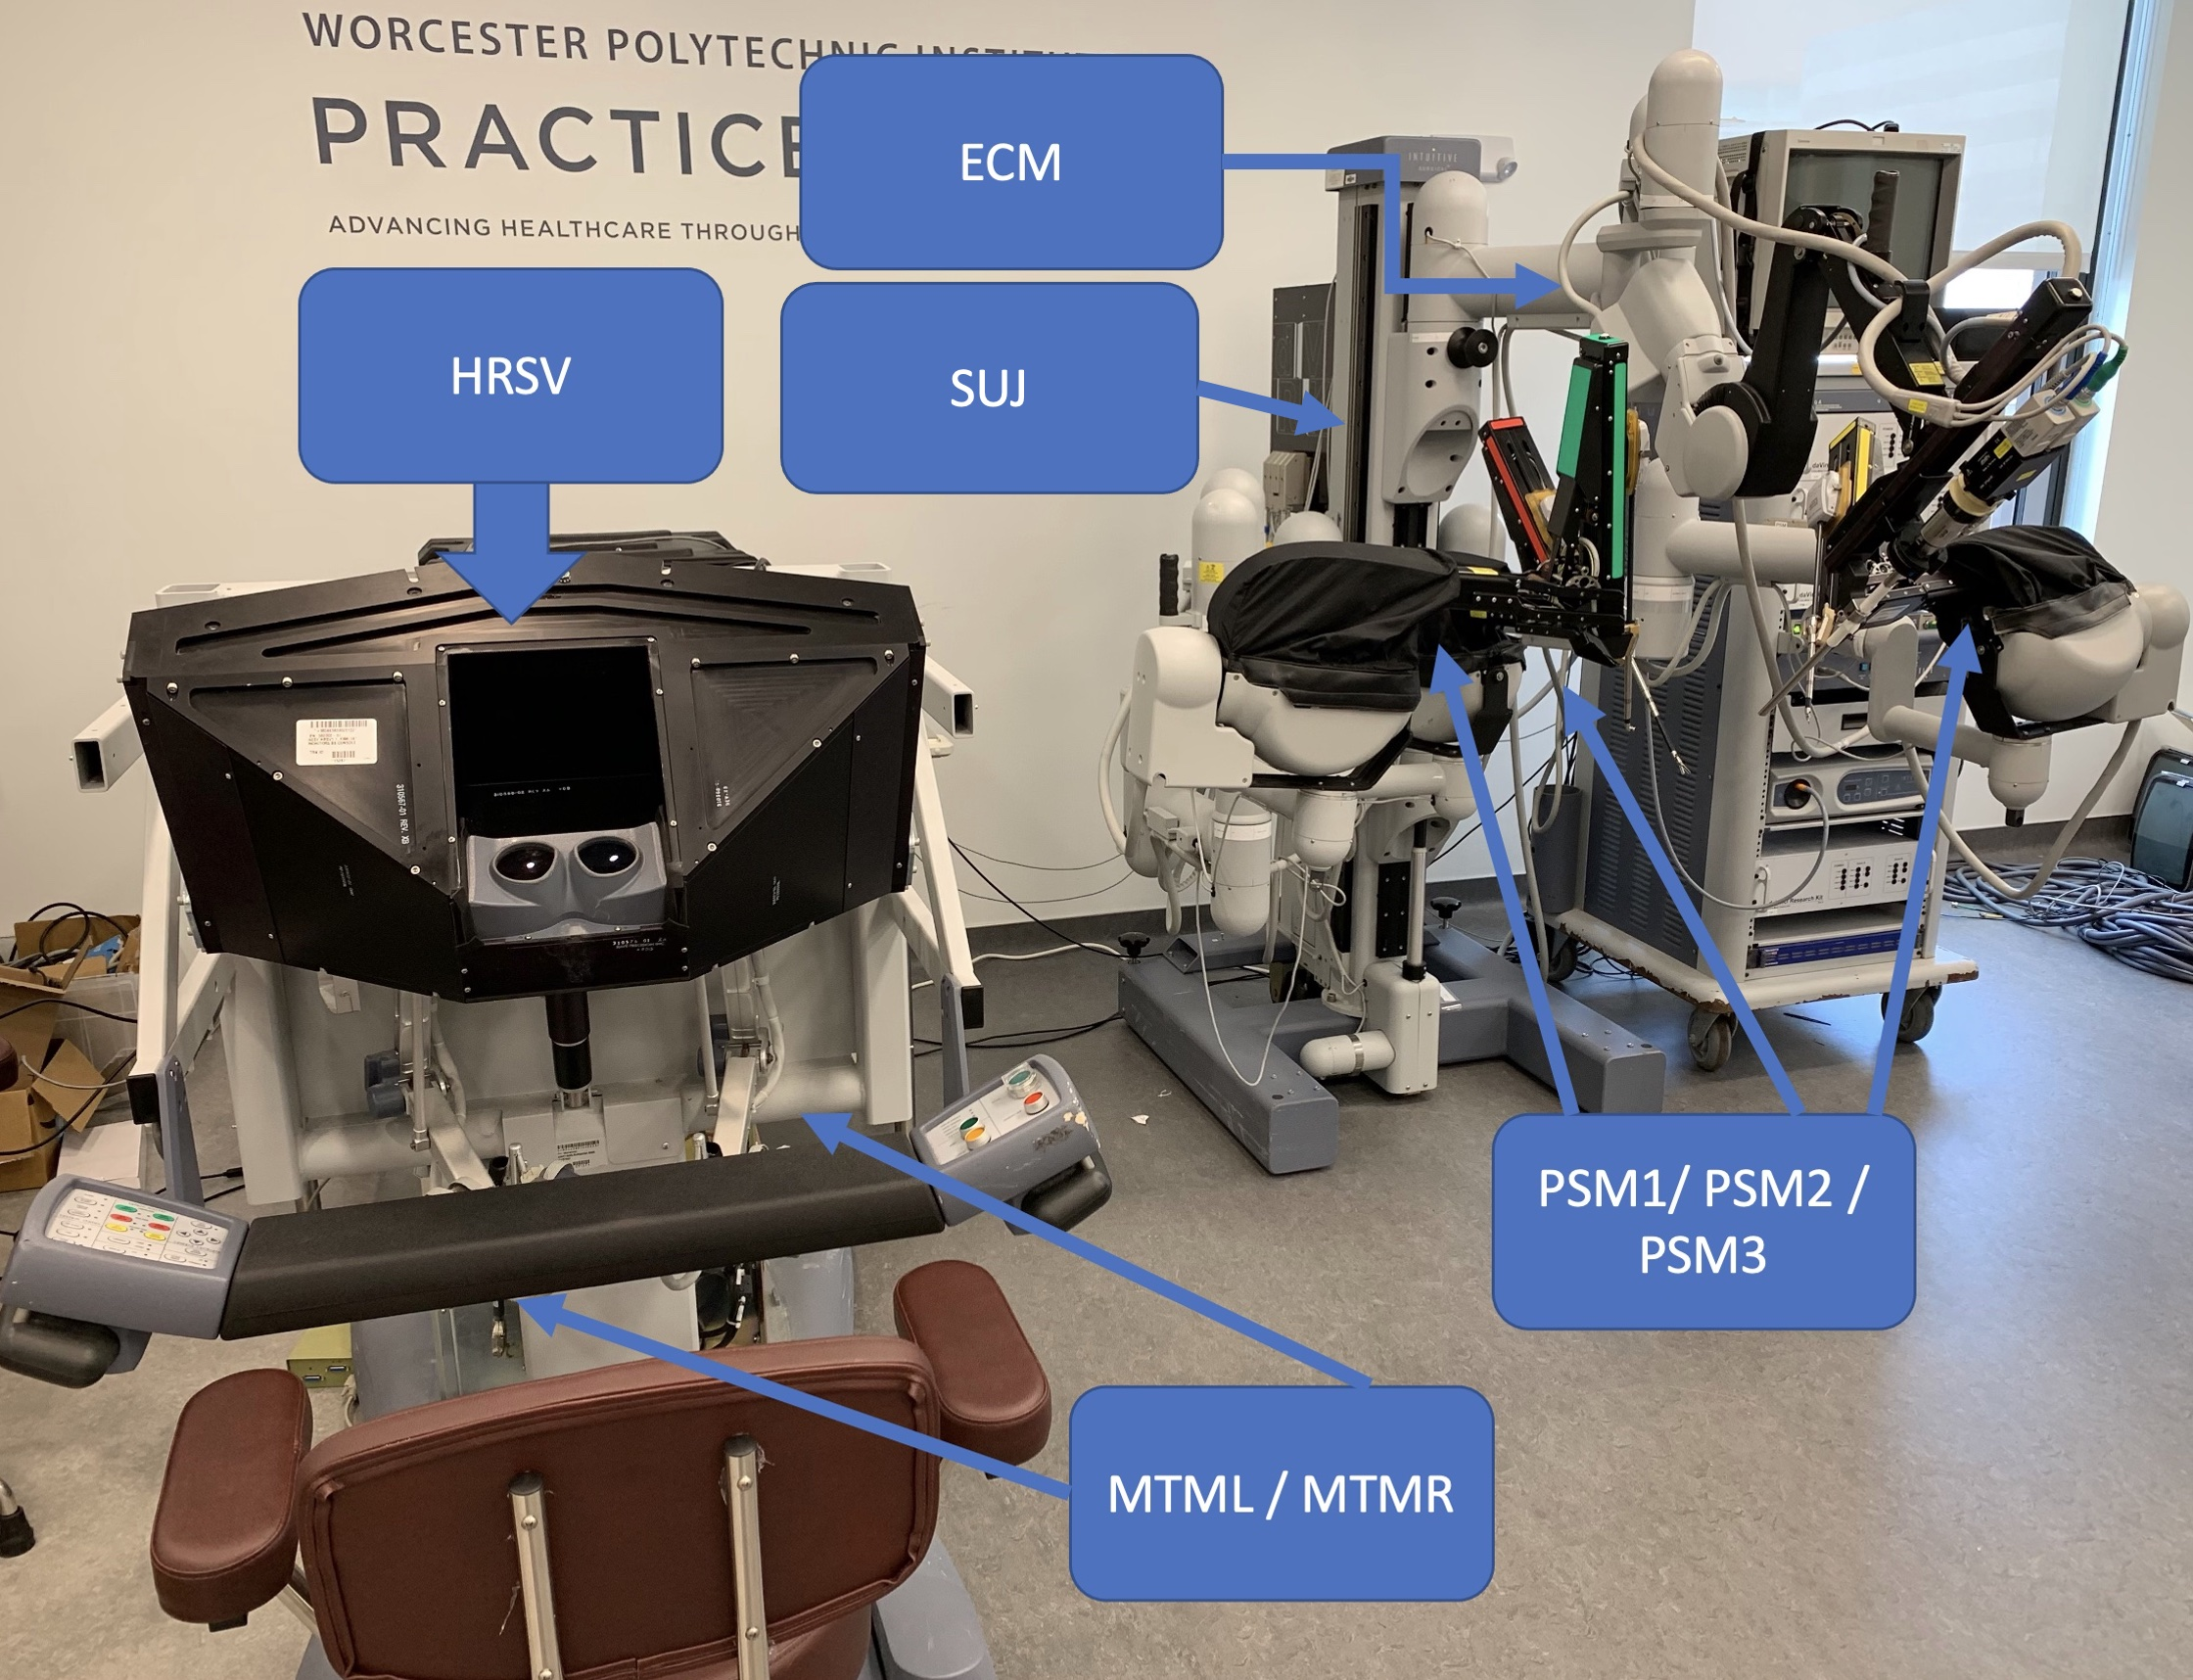
\includegraphics[width=0.95\linewidth]{figures/dVSS_intro.jpg}
    \caption{da Vinci surgical system}
    \label{fig:dVSS}
\end{figure}

\section{Document Conventions}

If you have any further questions, please feel free to check the GitHub discussion board at \url{https://github.com/jhu-dvrk/sawIntuitiveResearchKit/discussions}.

\section{Intended Audience and Reading Suggestions}

This is a tutorial for the starters of dVRK. Also, please check the Content list at the beginning for an overview.

\section{Product Scope}

This specification covers simple hardware and software setup. For advanced techniques, please check the websites given in the following section.

\section{References}

The whole specification is based on dVRK\cite{kazanzides2014open} and CRTK\cite{su2020collaborative} papers. And their corresponding GitHub repositories are:

\begin{itemize}
    \item da Vinci Research Kit (dVRK) ROS \\ Link: \url{https://github.com/jhu-dvrk/dvrk-ros}
    \item Collaborative Robotics Toolkit (CRTK) \\ Link: \url{https://github.com/collaborative-robotics/documentation/wiki}
    \item dVRK Wiki \\ Link: \url{https://github.com/jhu-dvrk/sawIntuitiveResearchKit/wiki/FirstSteps}
\end{itemize}


\chapter{Hardware Setup}
\label{ch: hardware}

This section is to introduce how to set up the dVRK in hardware level. This section would be helpful if you are a starter and the cables are unplugged. 

\section{Wire Connection}

\subsection{Daisy Chain (Power cable)}

This subsection is to set up the power system and integrate with the E-STOP. All the control boxes currently utilized have two connectors: one 4-pin connector and one 5-pin connect. A detailed wiring figure is shown in \autoref{fig:daisy}:

\begin{figure}[H]
    \centering 
    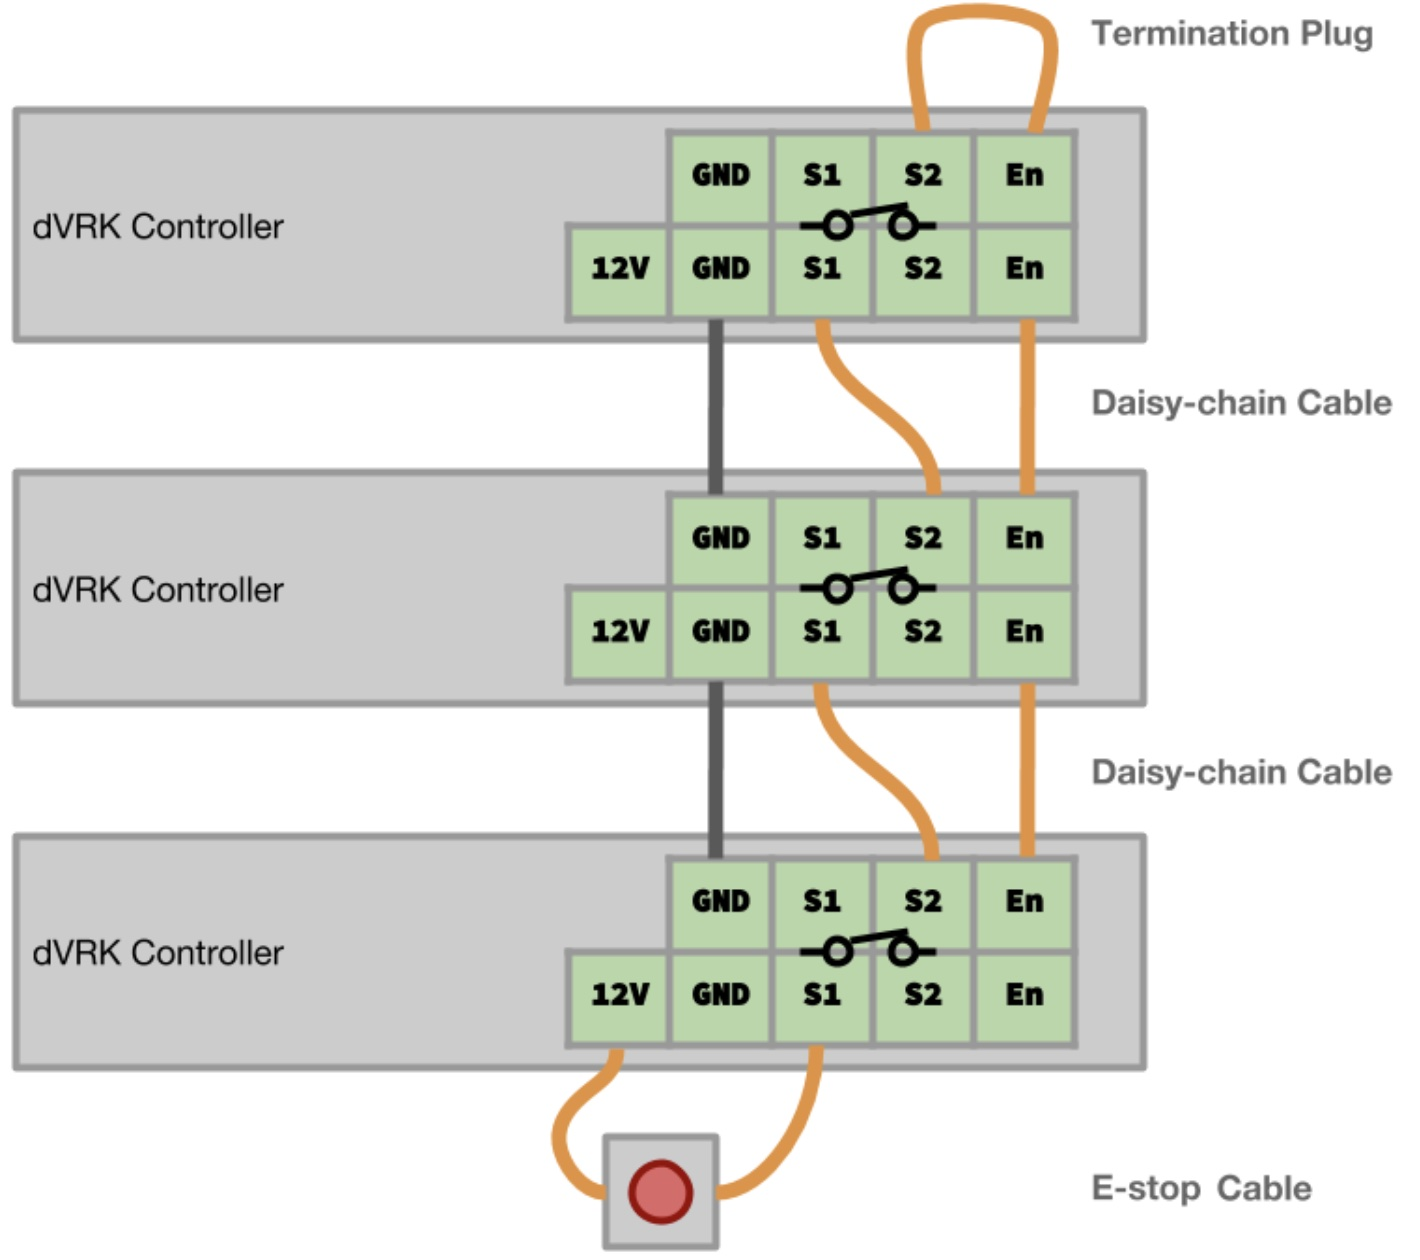
\includegraphics[width=0.7\linewidth]{figures/daisy_chain.jpg}
    \caption{dVRK daisy chain}
    \label{fig:daisy}
\end{figure}

\subsection{Firewire}

All the firewire connections should follow the listed rules:

\begin{itemize}
    \item input-output-input sequences shown in \autoref{fig:firewire}
    \item the overall connection between the work station and the control boxes should be through either the total input (for our case, MTML control box) or total output (for our case, SUJ control box)
    \item the board ID should be continuous ascending or descending (AKA, 0 $\rightarrow$ 12 or 12 $\rightarrow$ 0)
    \item To follow the control box board ID sequence, our control box connection sequence is MTML $\rightarrow$ MTMR $\rightarrow$ ECM $\rightarrow$ PSM1 $\rightarrow$ PSM2 $\rightarrow$ PSM3 $\rightarrow$ SUJ
\end{itemize}

\begin{figure}[H]
    \centering 
    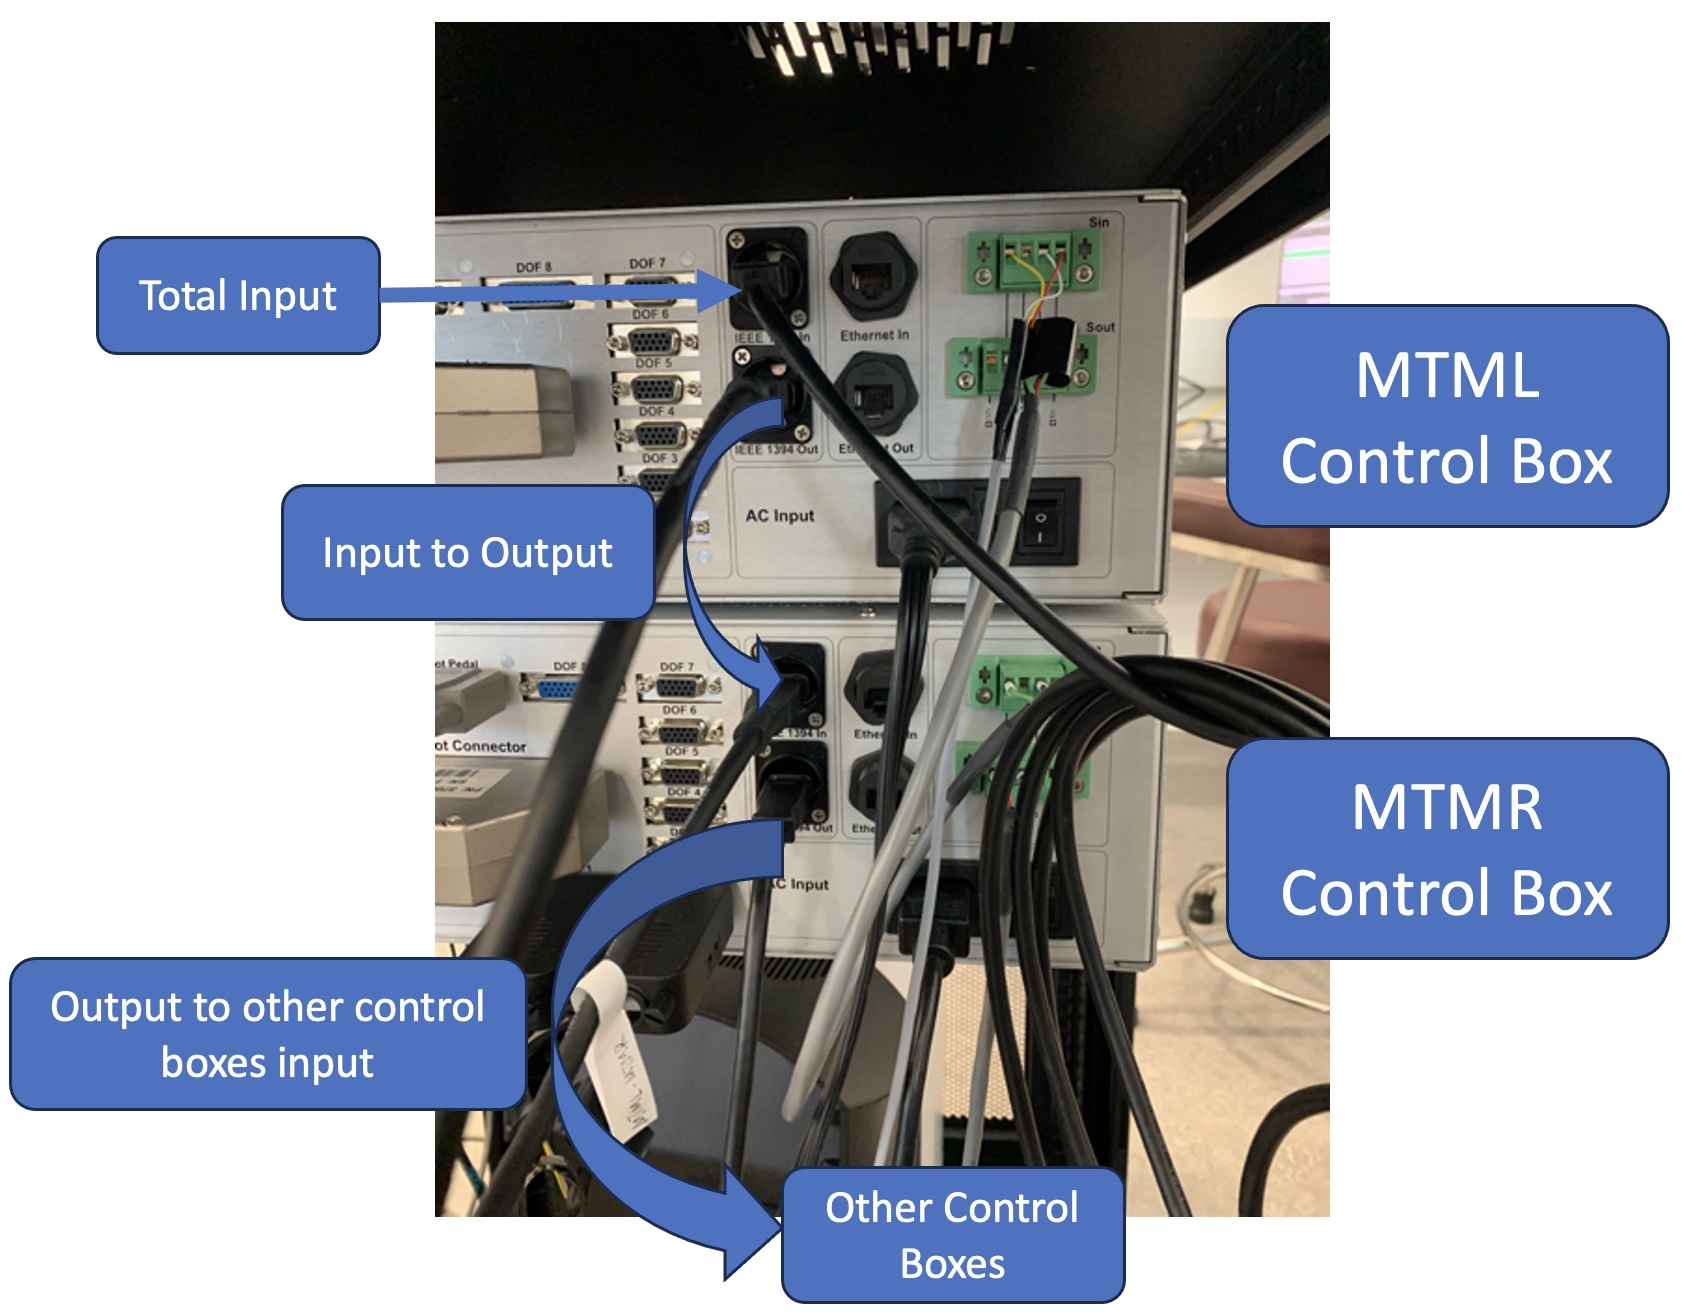
\includegraphics[width=0.9\linewidth]{figures/firewire_cable.jpg}
    \caption{Firewire Connection Example}
    \label{fig:firewire}
\end{figure}

Also, base on the fact that most computers does not have firewire port any more, you may need to buy a firewire card\footnote[1]{Currently Installed Firewire Card Purchase link: \url{https://www.amazon.com/gp/product/B002S53IG8/}}. For software level setup, please check \url{https://github.com/jhu-dvrk/sawIntuitiveResearchKit/wiki/Hardware#2-firewire} for more details. Generally, the software setup only needs to implement once for each computer.

\subsection{Foot Pedal}

The foot pedal is connected to MTMR control box as shown in \autoref{fig:foot_pedal}.

\begin{figure}[H]
    \centering 
    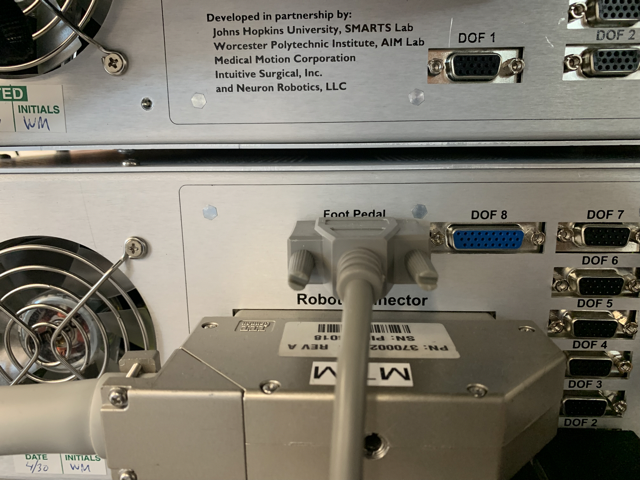
\includegraphics[width=0.7\linewidth]{figures/footpedal_port.png}
    \caption{Foot Pedal Connection}
    \label{fig:foot_pedal}
\end{figure}

If you need to make your own foot pedal, please check \url{https://github.com/jhu-dvrk/sawIntuitiveResearchKit/wiki/FootPedals} for details.

\subsection{Endoscope Focus Controller}

The endoscope focus controller is connected to MTMR control box as shown in \autoref{fig:endo_focus}. Please make sure the cable color is also the same as shown in \autoref{fig:endo_focus}.

\begin{figure}[H]
    \centering 
    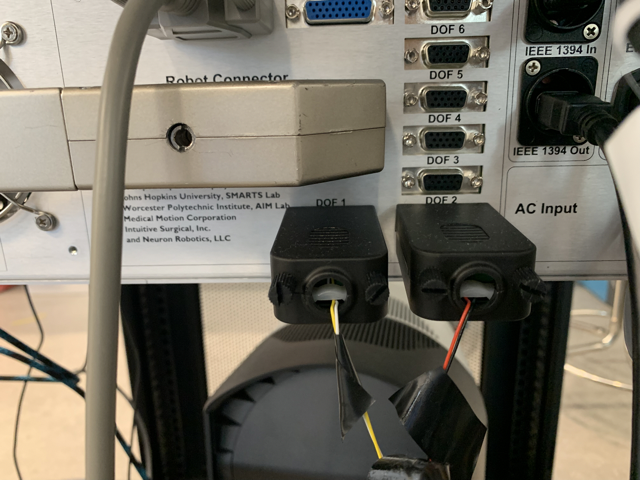
\includegraphics[width=0.7\linewidth]{figures/camera_focus.png}
    \caption{Endoscope Focus Controller Connection}
    \label{fig:endo_focus}
\end{figure}

The connection cable between dVRK control boxes and endoscope focus control box is a customized cable. For the details of cable construction and wiring instruction, please check \url{https://github.com/jhu-dvrk/sawIntuitiveResearchKit/wiki/Endoscope-Focus-Controller}.

\subsection{Ethernet UDP}

Even though we currently use firewire connection at WPI, Ethernet cable is also available for connections as shown in \autoref{fig:PC_connect}. We highly recommend to use firewire connections among control boxes for both methods.

\begin{figure}[H]
\centering
\subfloat[Firewire Connection]{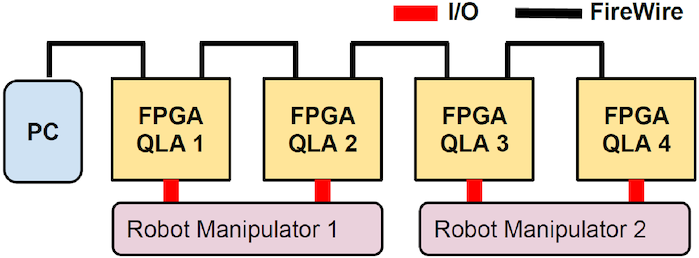
\includegraphics[width=0.45\linewidth]{figures/PC-FireWire-Controllers.png}
\label{fig_firewire_connect}}
\hfil
\subfloat[Ethernet Connection]{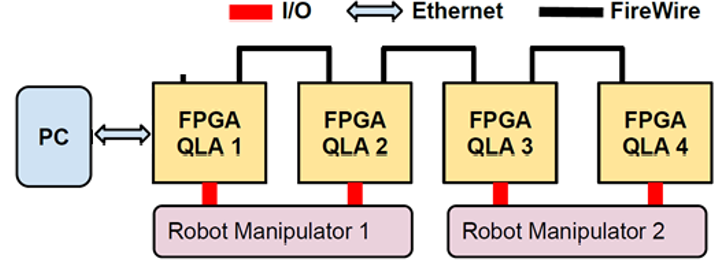
\includegraphics[width=0.45\linewidth]{figures/PC-Ethernet-Controllers.png}
\label{fig_ethernet_connect}}
\caption{Connections Between PC and Control Boxes}
\label{fig:PC_connect}
\end{figure}

If you are using Ethernet connection, please check \url{https://github.com/jhu-dvrk/sawIntuitiveResearchKit/wiki/ControllerConnection#ethernet-udp} for network setup details. In addition, it may include some configuration JSON file modifications or run code with the option \texttt{-pudp}.

\subsection{HRSV Video Pipeline}

Please check \url{https://github.com/jhu-dvrk/sawIntuitiveResearchKit/wiki/Video-Pipeline} for an introduction on how video pipeline works.

The principle behind the HRSV Video Pipeline Setup is to regard the two internal monitors embedded in the HRSV as two external monitors for connection and put the corresponding endoscope images into the monitors. 

For the internal monitors, we purchased some industrial monitors \footnote[2]{Monitor Purchase link: \url{https://www.beetronics.com/15-inch-monitor-flush-4-3}}. Those monitors fit the cavity at HRSV fairly well as shown in \autoref{fig:hrsv_monitor}:

\begin{figure}[H]
    \centering 
    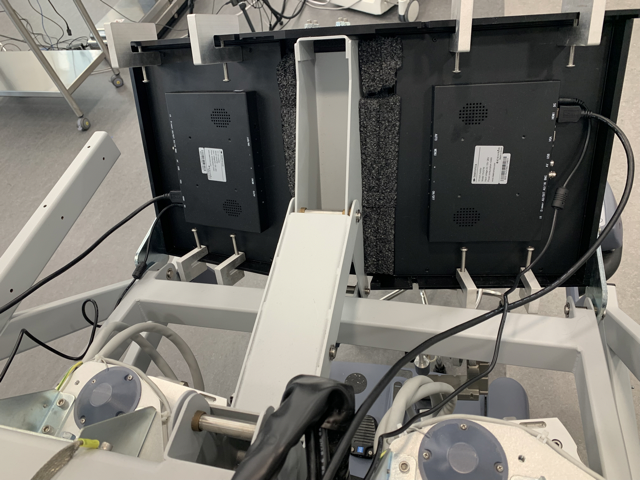
\includegraphics[width=0.55\linewidth]{figures/HRSV_sol.png}
    \caption{HRSV monitor replacement}
    \label{fig:hrsv_monitor}
\end{figure}

There are two common solutions for video streaming:

\subsubsection{SDI-to-USB3 Video Frame Grabber}

This method is currently leveraged at WPI. We purchased two epiphan SDI-to-USB3 frame grabbers \footnote[3]{SDI-to-USB3 Frame Grabber Purchase link: \url{https://www.epiphan.com/products/avio-sdi/}} shown in \autoref{fig:frame_grabber}. Those grabbers can convert the endoscope inputs to webcam inputs and thus it can be read by some ROS packages easily, such as ROS cv-camera package. Each camera require a separate frame grabber. Since each endoscope has two cameras, therefore at least two frame grabbers are required. If you would like to have a fixed connection via USB, it may require some basic knowledge on udev with Linux. Then, you may construct a customized udev rule for connection so that it can automatically detect the USB inputs with self-defined names. 

\begin{figure}[H]
    \centering 
    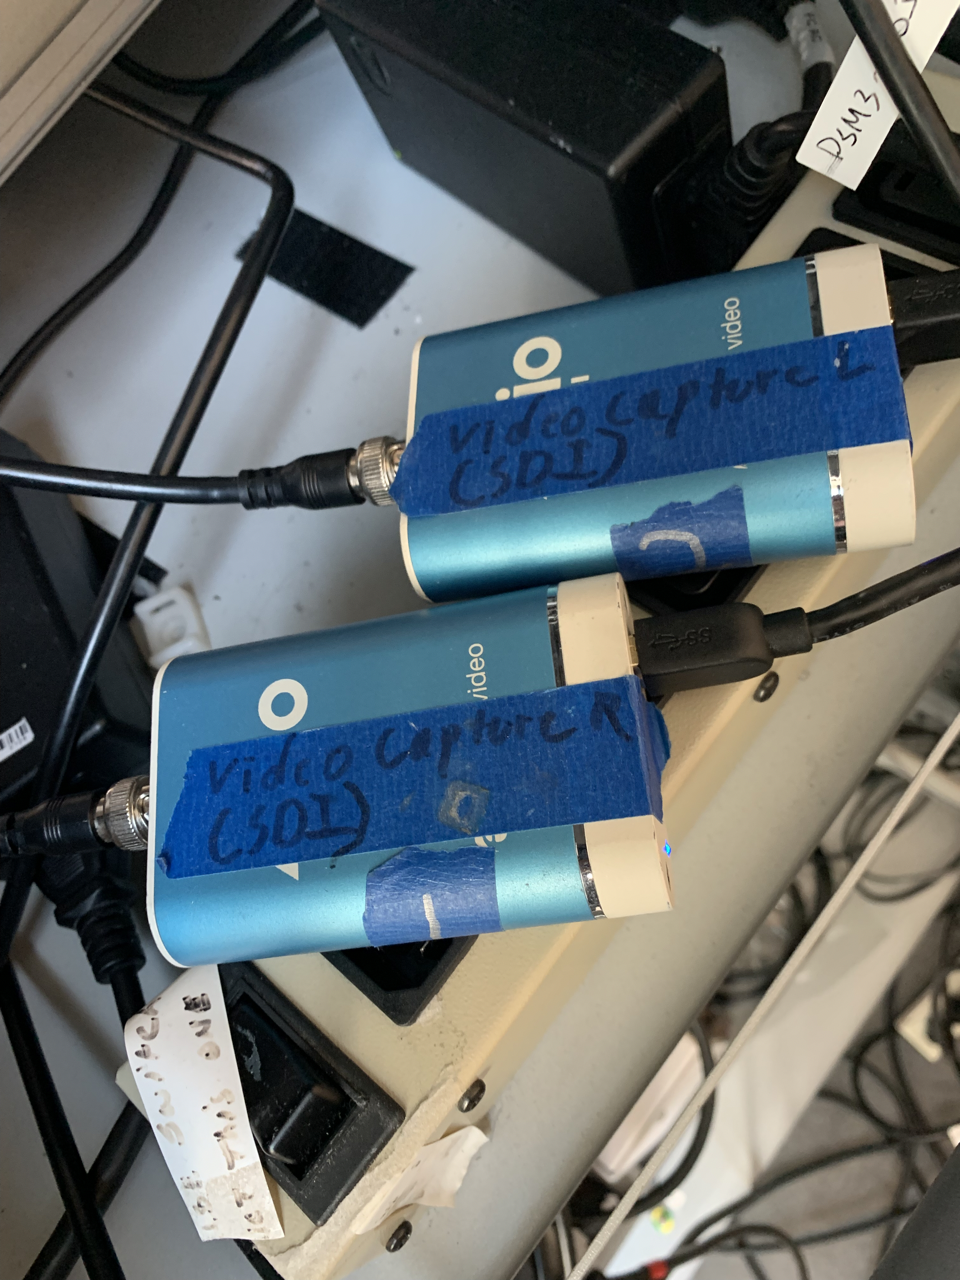
\includegraphics[width=0.6\linewidth]{figures/frame_grabber.png}
    \caption{Frame Grabber at WPI}
    \label{fig:frame_grabber}
\end{figure}

\subsubsection{DeckLink Duo Frame Grabber}

This solution is given by a subtopic under dVRK Wiki and currently utilized at Johns Hopkins University. Please check \url{https://github.com/jhu-dvrk/dvrk-ros/blob/devel/dvrk_robot/video.md} for details.

\subsection{Endoscope}

The endoscope needs to be connected to camera control units, focus control box and light source as shown in \autoref{fig:endoscope}. 

\begin{figure}[H]
\centering
\subfloat[Front View]{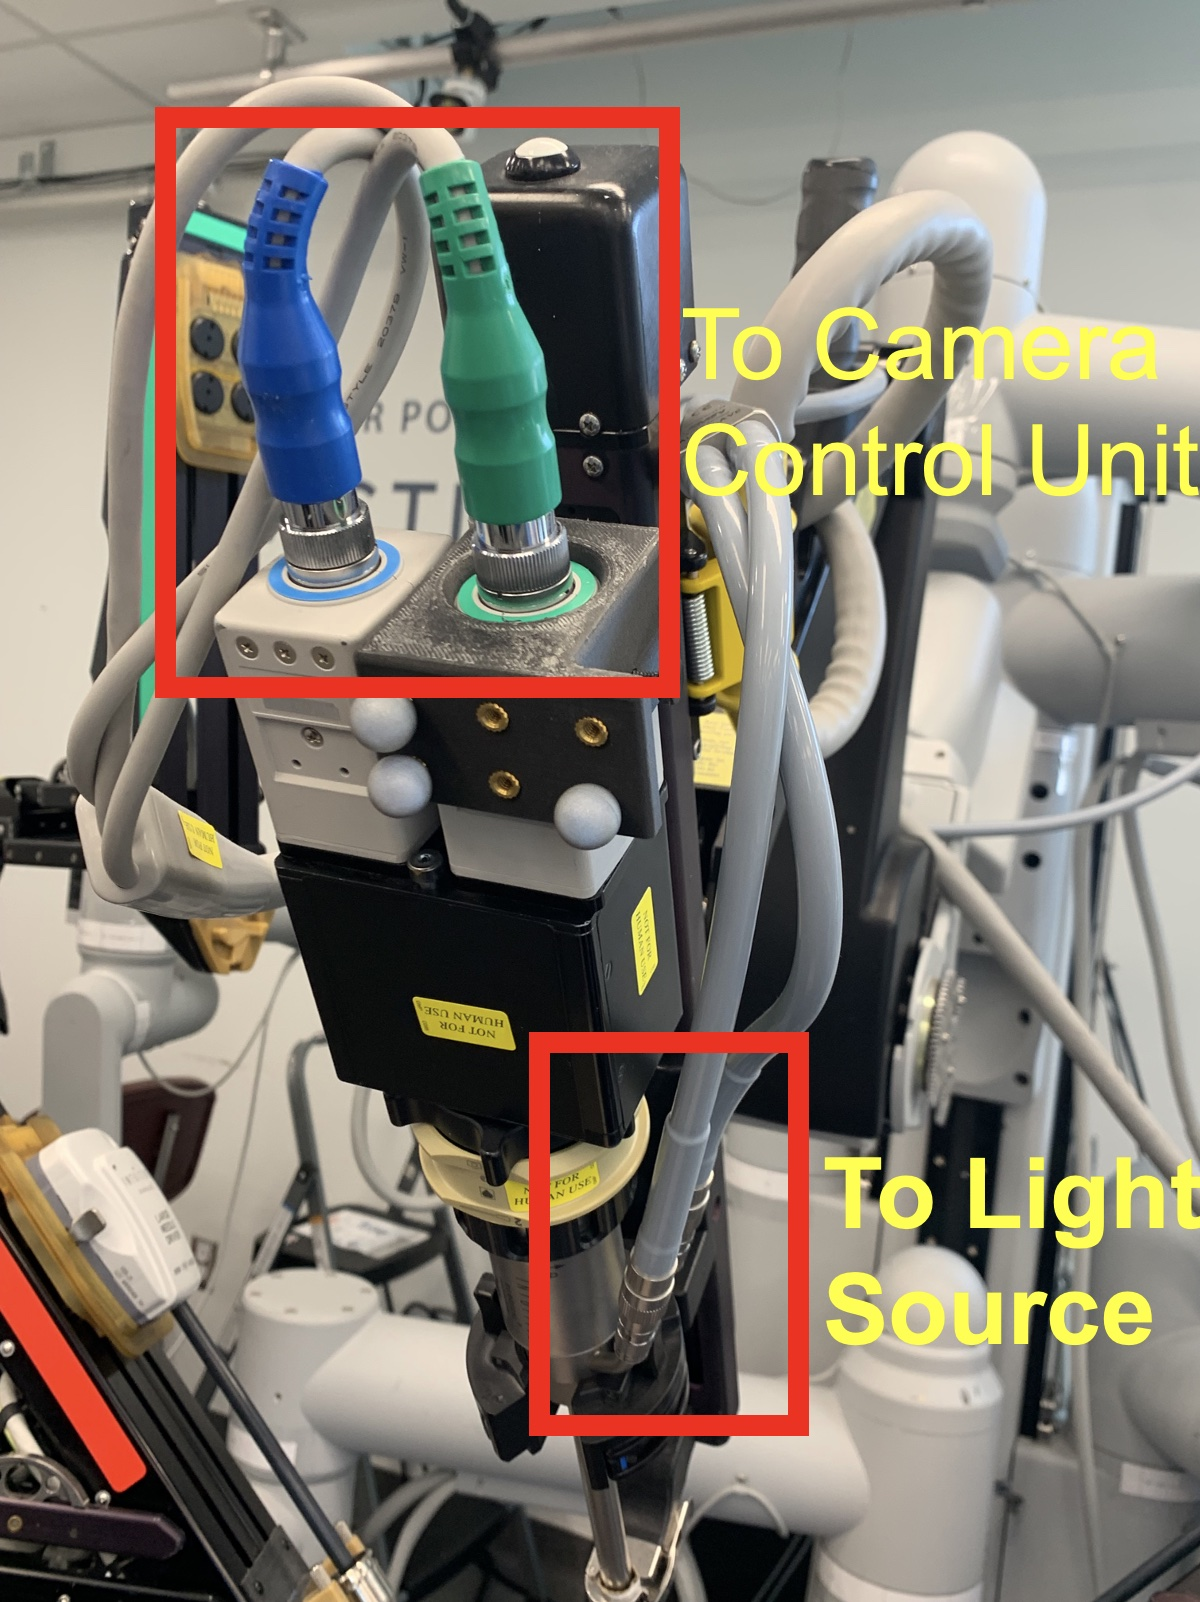
\includegraphics[width=0.45\linewidth, height=10cm]{figures/endo_cable1.jpg}}
\hfil
\subfloat[Side View]{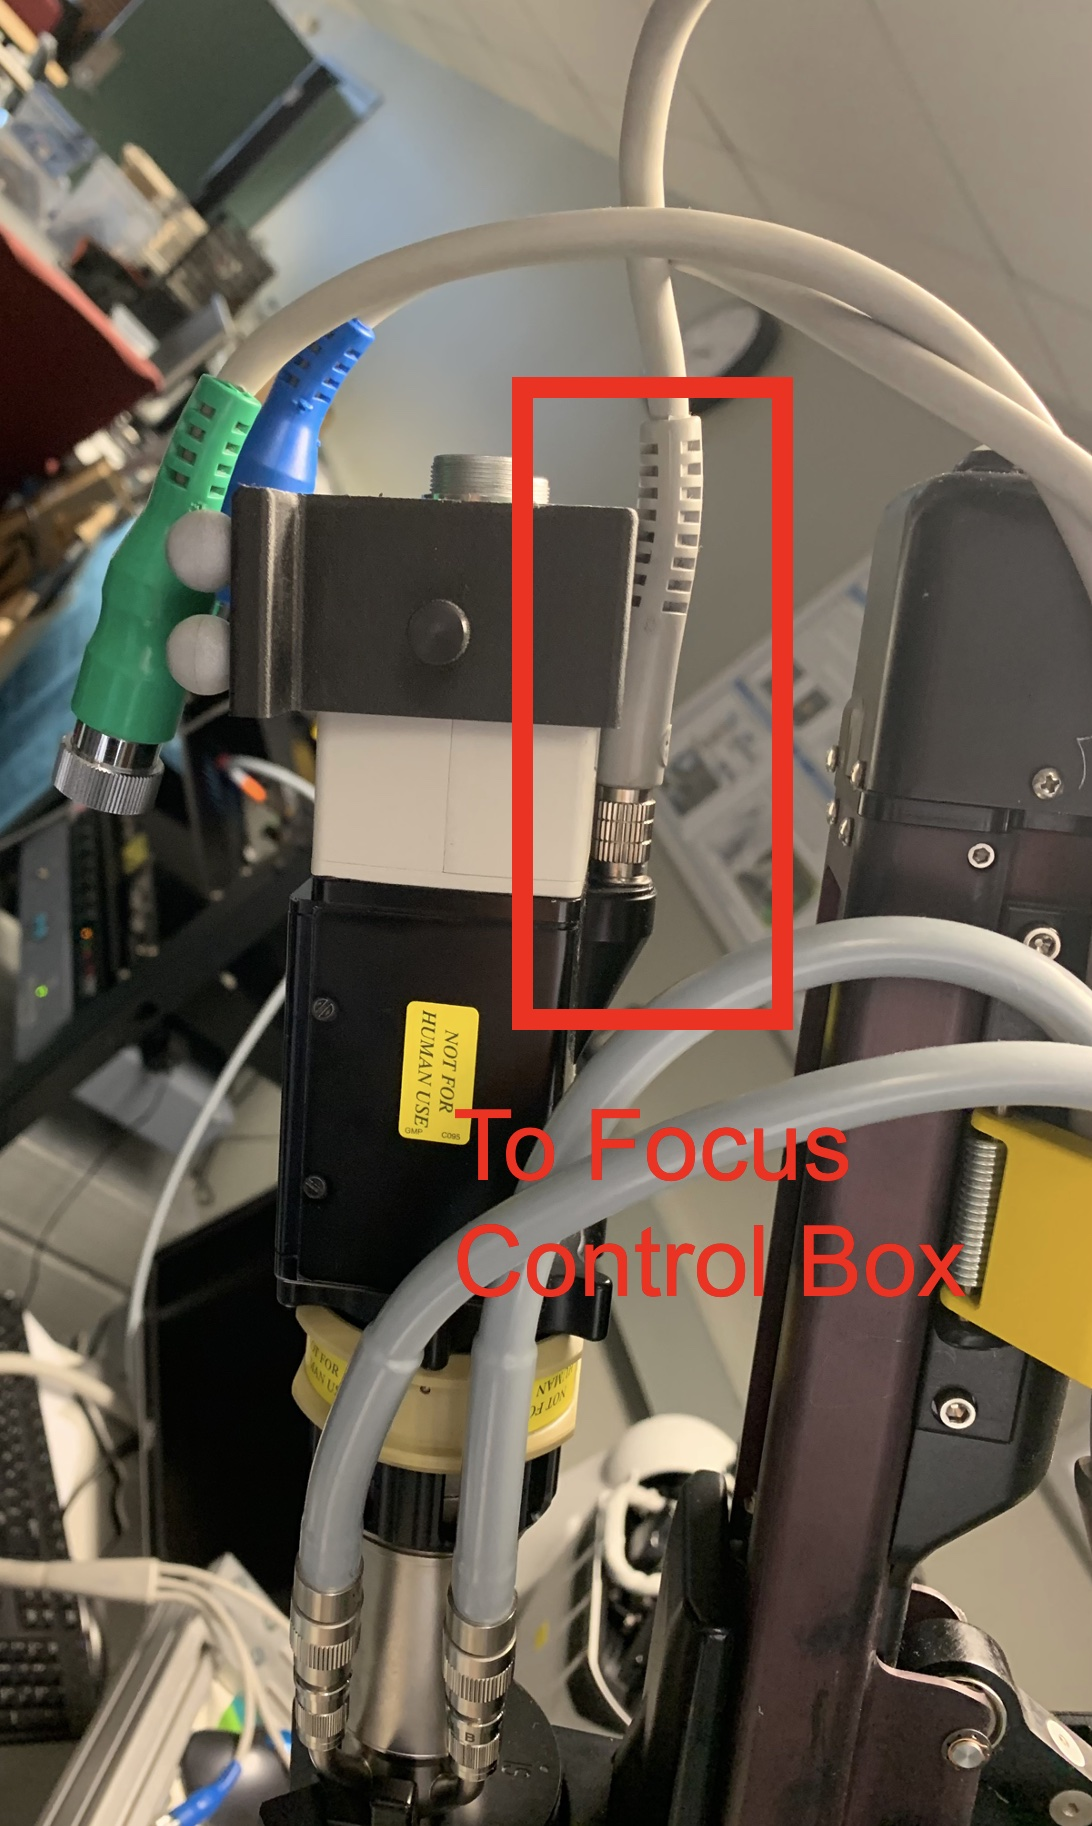
\includegraphics[width=0.45\linewidth, height=10cm]{figures/endo_cable2.jpg}}
\caption{Endoscope}
\label{fig:endoscope}
\end{figure}

Camera control units, focus control box and light source are all located at the control tower as show in \autoref{fig:endoscope_control}.

\begin{figure}[H]
\centering
\subfloat[Camera Control Unit (Upper) and Focus Control Box (Lower)]{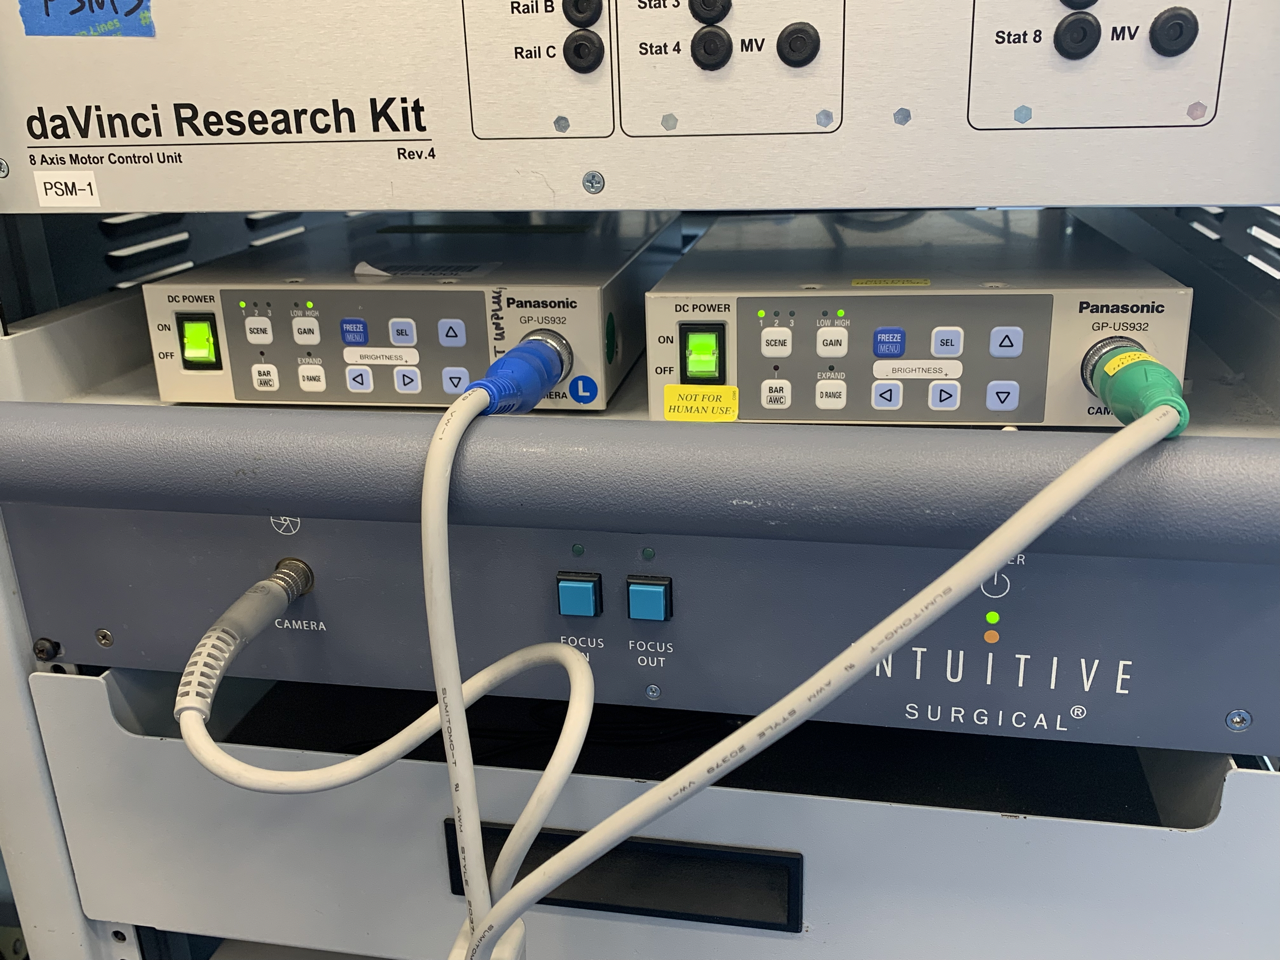
\includegraphics[width=0.45\linewidth]{figures/ccu_focus.png}}
\hfil
\subfloat[Light Source]{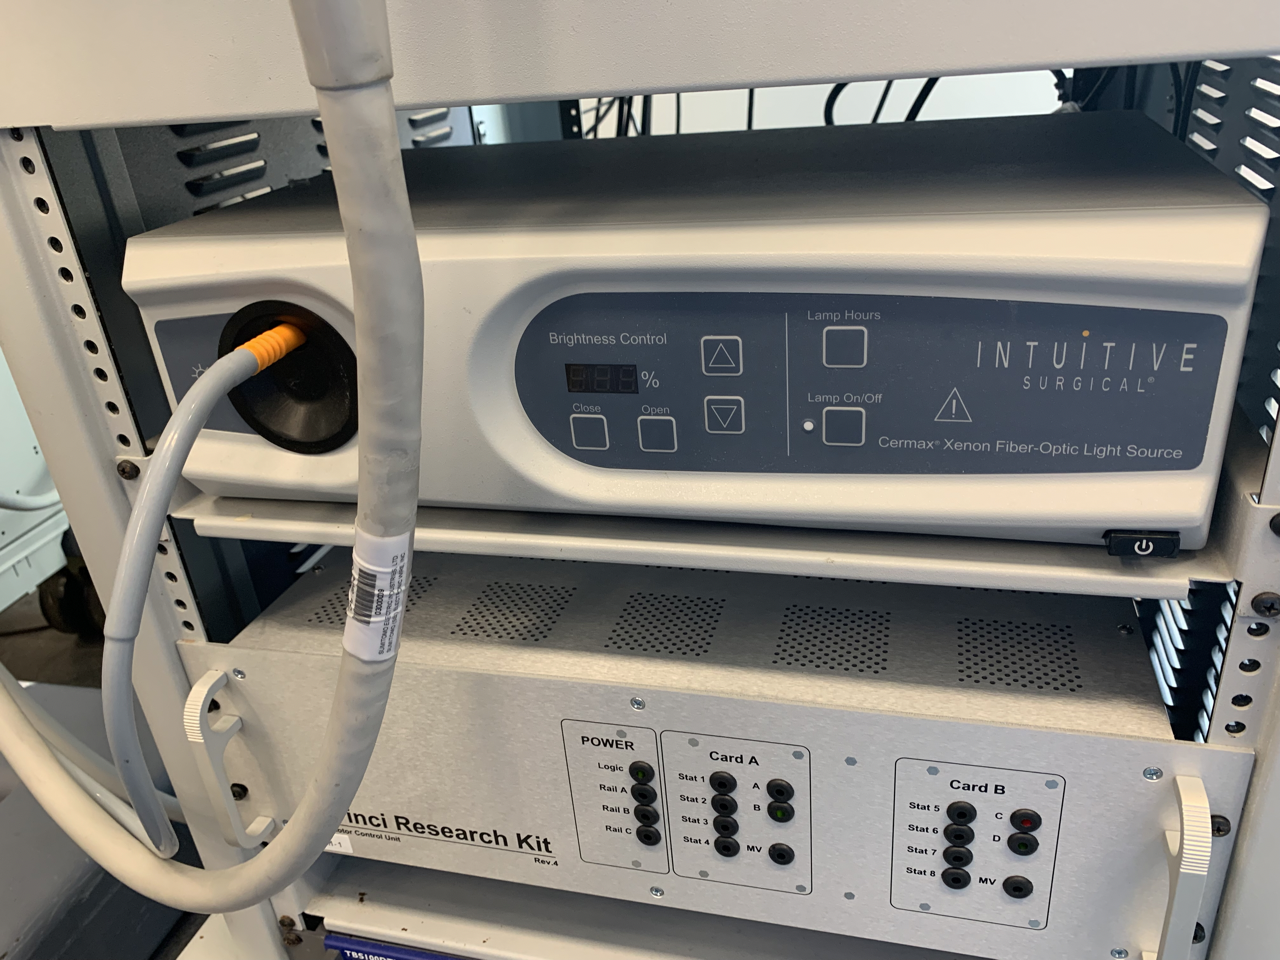
\includegraphics[width=0.45\linewidth]{figures/light_source.png}}
\caption{Endoscope Related Control Boxes on the Control Tower}
\label{fig:endoscope_control}
\end{figure}

\subsection{Other Hardware}

This section is for some hardware which has not been deployed at WPI dVRK setup.

\subsubsection{Head Sensor}

Head Sensor is a IR detector at HRSV outer shell as shown in \autoref{fig:head_sensor} . It can trigger the coag(mono) button as long as an optical obstacle was detected by the sensor. Please check \url{https://github.com/jhu-dvrk/sawIntuitiveResearchKit/wiki/HeadSensor} for details.

\begin{figure}[H]
    \centering 
    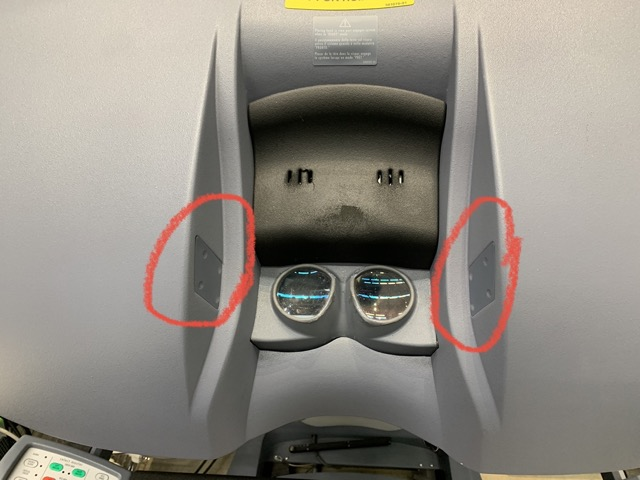
\includegraphics[width=0.5\linewidth]{figures/head_sensor.jpeg}
    \caption{HRSV Head Sensor}
    \label{fig:head_sensor}
\end{figure}


\section{Robot Initialize and Power Check}

Assume all the cables are connected correctly and all control boxes have been powered on.

\subsection{Emergency Stop Check}

Check the E-STOP and make sure it is released:

\begin{figure}[H]
    \centering
    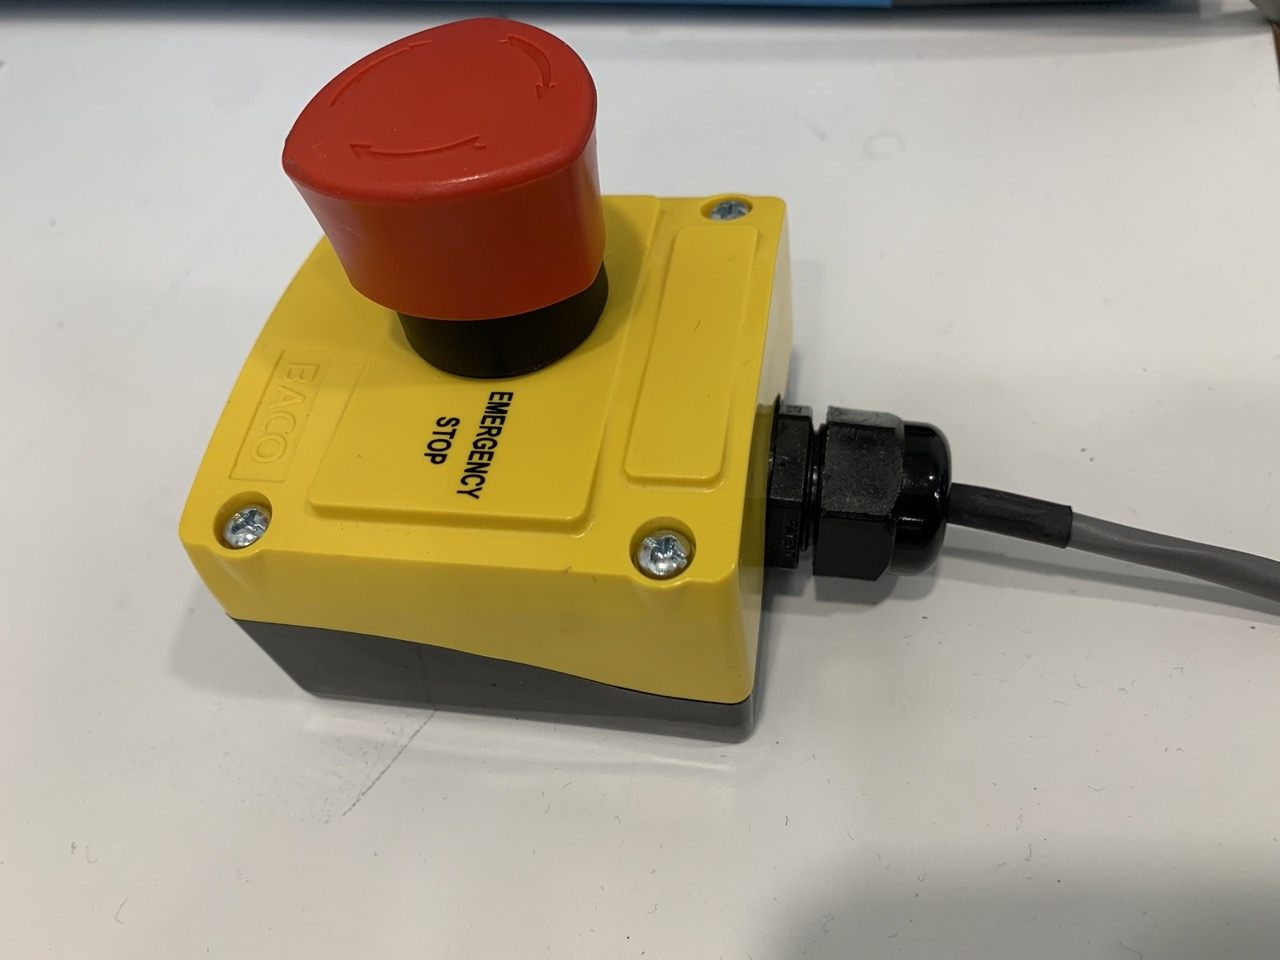
\includegraphics[width=0.45\linewidth]{figures/ESTOP_push.jpeg}
    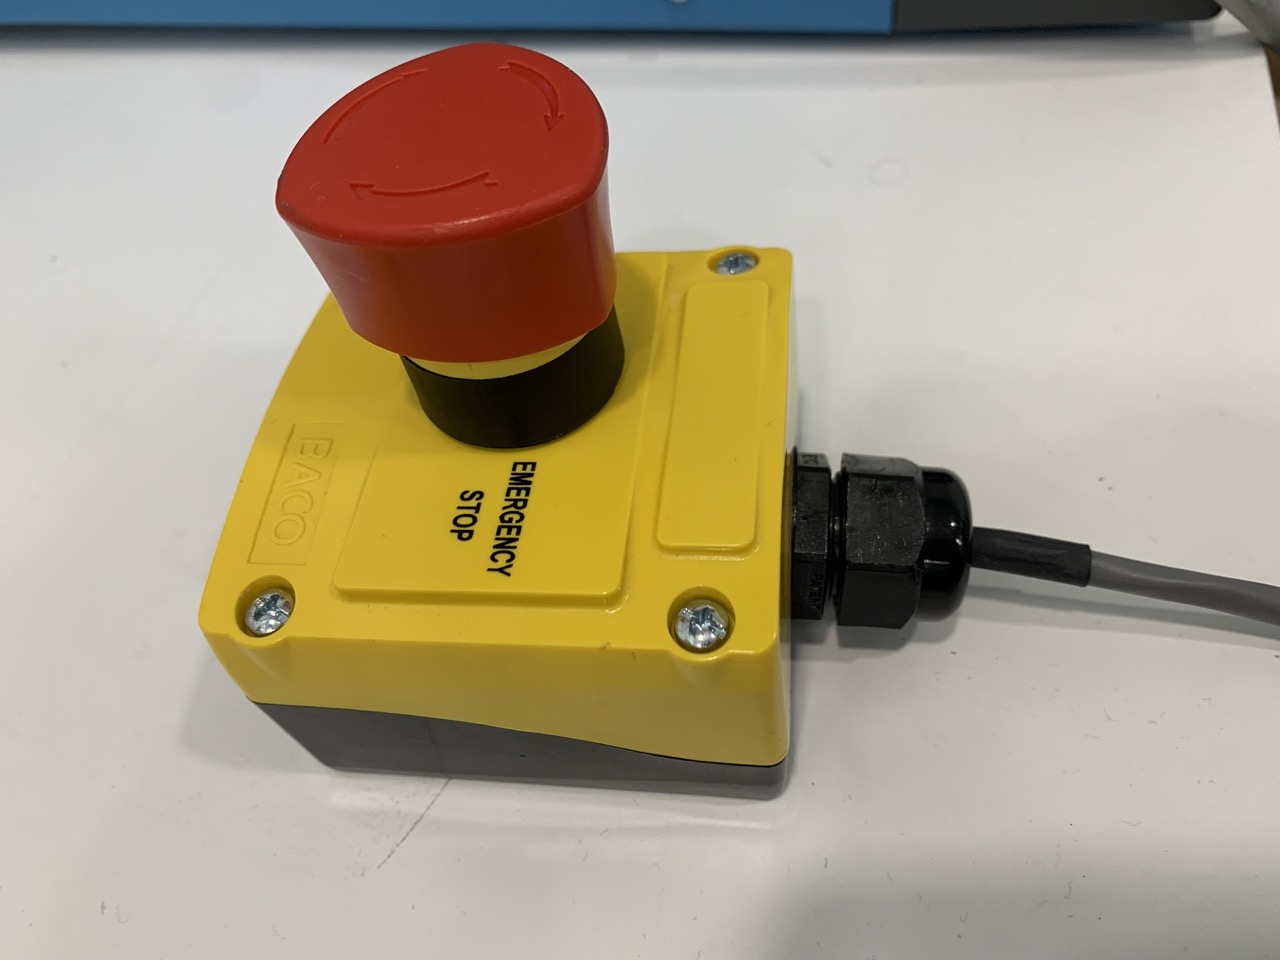
\includegraphics[width=0.45\linewidth]{figures/ESTOP_release.jpeg}
    \caption{E-stop pushed (left) and released (right)}
    \label{fig:ESTOP}
\end{figure}

When finishing using, please make sure to push the ESTOP down before leaving for safety consideration.

\subsection{Board ID Check}

Open a new terminal, run the following command:

\begin{minted}{bash}
    $ qladisp
\end{minted}

If you manage to get the following figure and find 13 board for total, you may move forward to next step:

\begin{figure}[H]
    \centering
    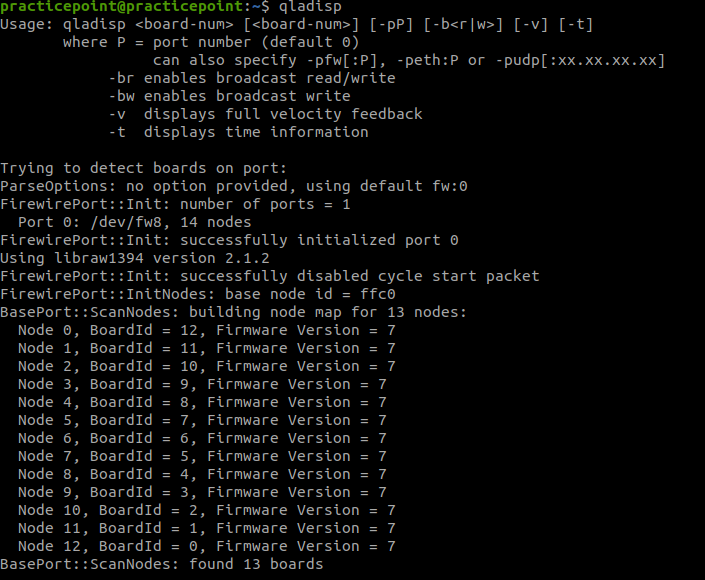
\includegraphics[width=0.5\linewidth]{figures/qladisp.png}
    \caption{expected terminal output for \texttt{qladisp} at WPI}
    \label{fig:qladisp}
\end{figure}

\texttt{qladisp} command can actually accomplish some additional tasks other than initialization confirmation. Please check \url{https://github.com/jhu-cisst/mechatronics-software/wiki/Example-Programs} for details.

\subsection{Robot Initialization}

If you have released the ESTOP (at the begining or recovering from emergency stop status), we highly recommend you to run the following command in a new terminal:

\begin{minted}{bash}
$ qlacommand -c close-relays
\end{minted}

This command is to enable the power of the control boxes. At the same time, you should hear the sound of activated fans. If not, please go back to check the cable connections, power and E-stop. This manual activation of power helps if the SUJ doesn't power on properly sometimes.

\section{Calibration}

Generally speaking, \textbf{you only do the calibration at the first time using the robot or when necessary (e.g. some arm misalignment problems [encoder reading and potentionmeter reading are inconsistent])}. You may skip this step if you have done the calibration in the past. We only introduce how to do the simplest current calibrations. For further calibrations, please refer to dVRK Wiki: \url{https://github.com/jhu-dvrk/sawIntuitiveResearchKit/wiki/Calibration}.

% or MTM has some misalignment as shown in the Q\&A section

Firstly, you need to direct to the dVRK configuration folder (Please check section 3.1 for more information).

% \begin{minted}{bash}
%     $ cd
%     $ cd catkin_ws_dvrk/src/cisst-saw/sawIntuitiveResearchKit/share/wpi-triad
% \end{minted}

Before calibration, you should ensure that your relays are closed. If not, open a new terminal and run following command:

\begin{minted}{bash}
$ qlacommand -c close-relays
\end{minted}

At the same time, you should hear the sound of activated fans. If not, please go back to check the cable connections, power and E-STOP.

Alternatively, you can also generate new xml for the given .cal from Intuitive Surgical as instructed in \url{https://github.com/jhu-dvrk/sawIntuitiveResearchKit/wiki/XMLConfig}.

\subsection{SUJ Current Calibration}

Go back to the terminal which is directed to the dVRK configuration folder and run:

\begin{minted}{bash}
$ sawRobotIO1394CurrentCalibration -c sawRobotIO1394-SUJ.xml
\end{minted}

Follow the instruction in the code and replace the \texttt{sawRobotIO1394-SUJ.xml} with the calibrated xml file.

For advanced SUJ calibration (usually only need to do once), please check \url{https://github.com/jhu-dvrk/sawIntuitiveResearchKit/wiki/SUJ}.

\subsection{PSM Current Calibration}

\textbf{Firstly, make sure your detachable surgical tools are not installed on the PSM when calibration}

Then, go back to the terminal which is directed to the dVRK configuration folder and run:

\begin{minted}{bash}
$ sawRobotIO1394CurrentCalibration -c sawRobotIO1394-PSM2-29996.xml 
\end{minted}

Follow the instruction in the code and replace the \texttt{sawRobotIO1394-PSM2-29996.xml} with the calibrated xml file.

For the other PSMs, they share the identical procedures. You only need to modify the PSM number and corresponding series number.

\subsection{ECM Current Calibration}

Open a new terminal, direct to the dVRK configuration folder and run:

\begin{minted}{bash}
$ sawRobotIO1394CurrentCalibration -c sawRobotIO1394-ECM-25975.xml 
\end{minted}

Follow the instruction in the code and replace the \texttt{sawRobotIO1394-ECM-25975.xml} with the calibrated xml file. You only need to modify your ECM serial number if you are not using WPI clinical da Vinci.

For ECM advanced calibration(usually only need to do once), please check \url{https://github.com/jhu-dvrk/sawIntuitiveResearchKit/wiki/ECM}.

\subsection{MTM Current Calibration}

Open a new terminal, direct to the dVRK configuration folder and run:

\begin{minted}{bash}
$ sawRobotIO1394CurrentCalibration -c sawRobotIO1394-MTML-33100.xml 
\end{minted}

Follow the instruction in the code and replace the \texttt{sawRobotIO1394-MTML-33100.xml} with the calibrated xml file.

For the other MTMs, they share the identical procedures. You only need to modify the MTML/R and corresponding series number.

For MTM advanced calibration, please check \url{https://github.com/jhu-dvrk/sawIntuitiveResearchKit/wiki/Calibration#gripper-on-mtms}. For WPI clinical da Vinci, you don't have to do this calibration since we have mechanically lubricate and adjust some detachable surgical tools to make them grasp objects tightly.

\section{Tool Deployment}

Tool deployment includes two parts: tool detection and tool installation.

For tool detection, there are three models: 

\begin{itemize}
    \item Automatic: let the tool pedal auto-detect the tool type from the chip embedded in the tool
    \item Manual: select tool type manually
    \item Fixed: pre-selected fixed tool type for the arm
\end{itemize}

For tool installation, the major concern is the alignment of the tool and the tool pedal as shown in \autoref{fig:tool_attach}.

\begin{figure}[H]
    \centering
    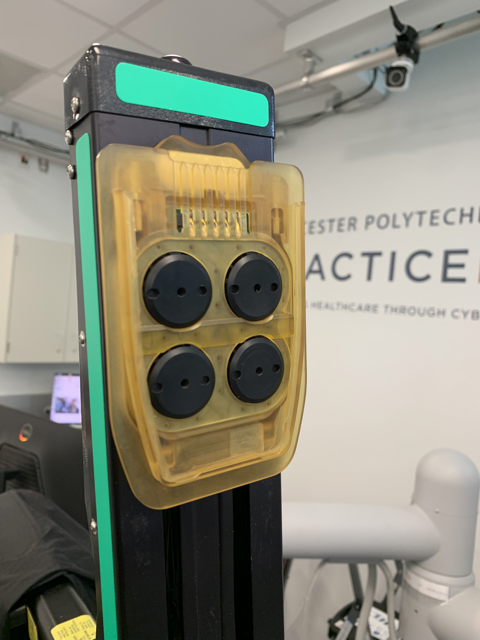
\includegraphics[width=0.45\linewidth]{figures/tool_pedal.png}
    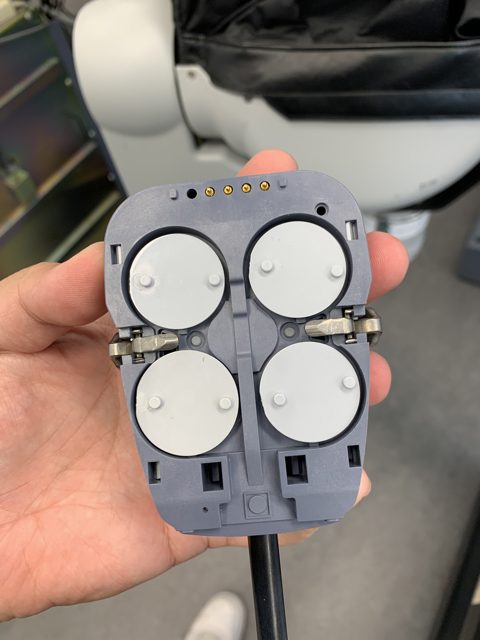
\includegraphics[width=0.45\linewidth]{figures/tool_back.png}
    \caption{Alignment of the rotating pans between the tool pedal and the tool}
    \label{fig:tool_attach}
\end{figure}

For our cases at WPI, we are currently using Manual model for tool detection. Therefore, please select your preferred tool and install it on the PSM before you activate da Vinci system. You may put the tool pedal around the home position shown in \autoref{fig:tool_attach} for an easier installation. If you select to use Automatic model, you may power on the system firstly and home the robot, then you can attach the tool to the arm and the tool information will be automatically detected. Nevertheless, if you have a customized tool, Manual model is required.

\newpage

\chapter{Software and Applications}
\label{ch: Software}

\section{dVRK Configuration Folder Path}

Before starting working on this section, you need to accomplish the construction of ROS work space. The work space name shown in the following sections are the names currently used in WPI local environment. You are free to modify the name based on your personal preference.

\subsection{ROS 1}

For ROS 1, an instruction of building ROS work space is shown in the following link \url{https://github.com/jhu-dvrk/sawIntuitiveResearchKit/wiki/CatkinBuild}.

\subsubsection{Master Branch}

For sawIntuitiveResearchKit repository in master branch, you can run following commands in a new terminal to be directed to the dVRK configuration folder path:

\begin{minted}{bash}
    cd ~/catkin_ws_dvrk/src/cisst-saw/sawIntuitiveResearchKit/share
\end{minted}

In this folder, you can see all shared configurations from different universities. 

For instance, at WPI, you would need to head to \texttt{wpi\_test} folder for more specific configuration JSON files.

You may refer to JHU configuration JSON files to create your own JSON files.

\subsubsection{Develop Branch}

For sawIntuitiveResearchKit repository in master branch, you can run following commands in a new terminal to be directed to the dVRK configuration folder path:

\begin{minted}{bash}
    cd ~/catkin_ws_dvrk_devel/src/cisst-saw/sawIntuitiveResearchKit/share
\end{minted}

In this folder, you can see all shared configurations from different universities. 

For instance, at WPI, you would need to head to \texttt{wpi\_test} folder for more specific configuration JSON files.

You may refer to JHU configuration JSON files to create your own JSON files.

\subsection{ROS 2}

For ROS 2, an instruction of building ROS work space is shown in the following link \url{https://github.com/jhu-dvrk/sawIntuitiveResearchKit/wiki/BuildROS2}.

For the configuration folder, you may need to work on your own to create your own configuration JSON files, which requires some knowledge of the software architecture. You may also refer to JHU ROS2 configuration JSON files in \url{https://github.com/dvrk-config/dvrk_config_jhu}. 

For instance, at WPI, you can run following commands in a new terminal to be directed to the dVRK configuration folder path:

\begin{minted}{bash}
    cd ~/ros2_ws/install/dvrk_config_wpi
\end{minted}

\subsection{Undertand JSON Configuration File}

You can check the existed configuration files as reference. Moreover, you can check this link \url{https://dvrk.lcsr.jhu.edu/documentation/schemas/v2.1/dvrk-console.html} to learn about the meanings of the parameters.

\subsection{Switch between ROS 1 and ROS2}

Generally speaking, source both ROS1 and ROS2 at \texttt{bashrc} is not recommended at Ubuntu 20.04. Therefore, as a solution, you can source one of the two ROS version at one time as shown in \autoref{fig:ros_switch}.

\begin{figure}[H]
    \centering
    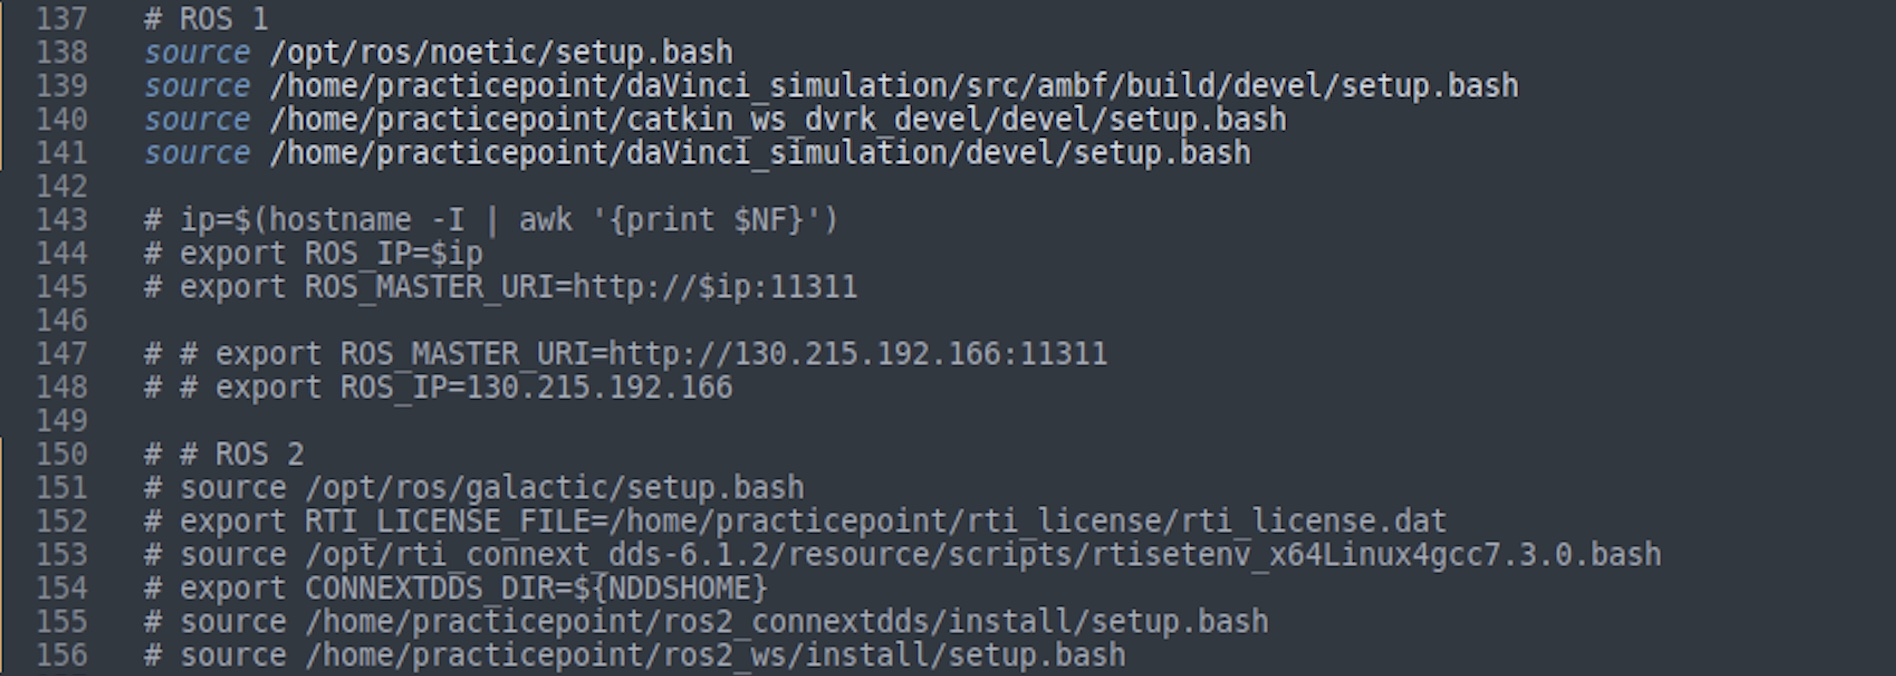
\includegraphics[width=0.9\linewidth]{figures/ROS_switch_bash.jpg}
    \caption{sections in the bashrc file for ROS1 and ROS2 source}
    \label{fig:ros_switch}
\end{figure}

\begin{itemize}
    \item ROS 1 : Comment line 151, 155 and 156; Uncomment line 138-141
    \item ROS 2: Uncomment line 151, 155 and 156; Comment line 138-141
\end{itemize}

\section{Activate dVRK}

\subsection{ROS 1}

Open a new terminal, run following command to run ROS:

\begin{minted}{bash}
$ roscore
\end{minted}

Create a new terminal which is directed to the dVRK configuration folder as shown in section 3.1.1 and run:

\begin{minted}{bash}
$ rosrun dvrk_robot dvrk_console_json -j console-[code name].json -p [timestep]
\end{minted}
where
\begin{equation*}
    timestep = \frac{1}{desired \, frequency}
\end{equation*}

Here is the table introducing different code names:

\begin{table}[H]
    \centering
    \begin{tabular}{|c|c|}
    \hline
    % \multicolumn{12}{|c|}{N = 11, $\alpha$ = 0.8, one-turn play} \\
    % \hline
    Code Name & Purpose \\
    \hline
    ECM, MTML/R, PSM 1/2/3 & Activate corresponding arms \\
    \hline
    ECM-MTML-MTMR-Teleop & Teleoperate ECM with two MTMs \\
    \hline
    MTML-MTMR & \makecell{Activated two MTMs \\ usually use when teleoperation in AMBF simulation \cite{munawar2022open}} \\
    \hline
    SUJ & \makecell{Activate SUJ to manually move PSM 1\&2 and ECM \\ with respect to SUJ}\\
    \hline
    SUJ-PSM3 & Activate SUJ and PSM3 so all PSMs can move\\
    \hline
    SUJ-ECM-PSM & \makecell{Activate SUJ, ECM and PSM3 \\ so that all arms can move} \\
    \hline
    SUJ-MTMR-PSM1-Teleop & Teleoperate PSM1 with MTMR \\
    \hline
    SUJ-ECM-MTMR-PSM1-MTML-PSM3-Teleop & \makecell{Teleoperate two arms with two MTMs \\ utilized in the suture user study} \\
    \hline
    \makecell{SUJ-ECM-MTMR-PSM1-\\-MTML-PSM2-PSM3-Teleop} & \makecell{Full system activated with \\  teleoperation of all three PSMs enabled}  \\
    % \hline
    % SUJ-MTML-PSM2-Teleop-Custom & Enable teleopeartion with MTM  \\
    \hline
    \end{tabular}
    \caption{code name table}
    \label{tab:code_name}
\end{table}

After running the above code, you should enter a GUI looks like:

\begin{figure}[H]
    \centering
    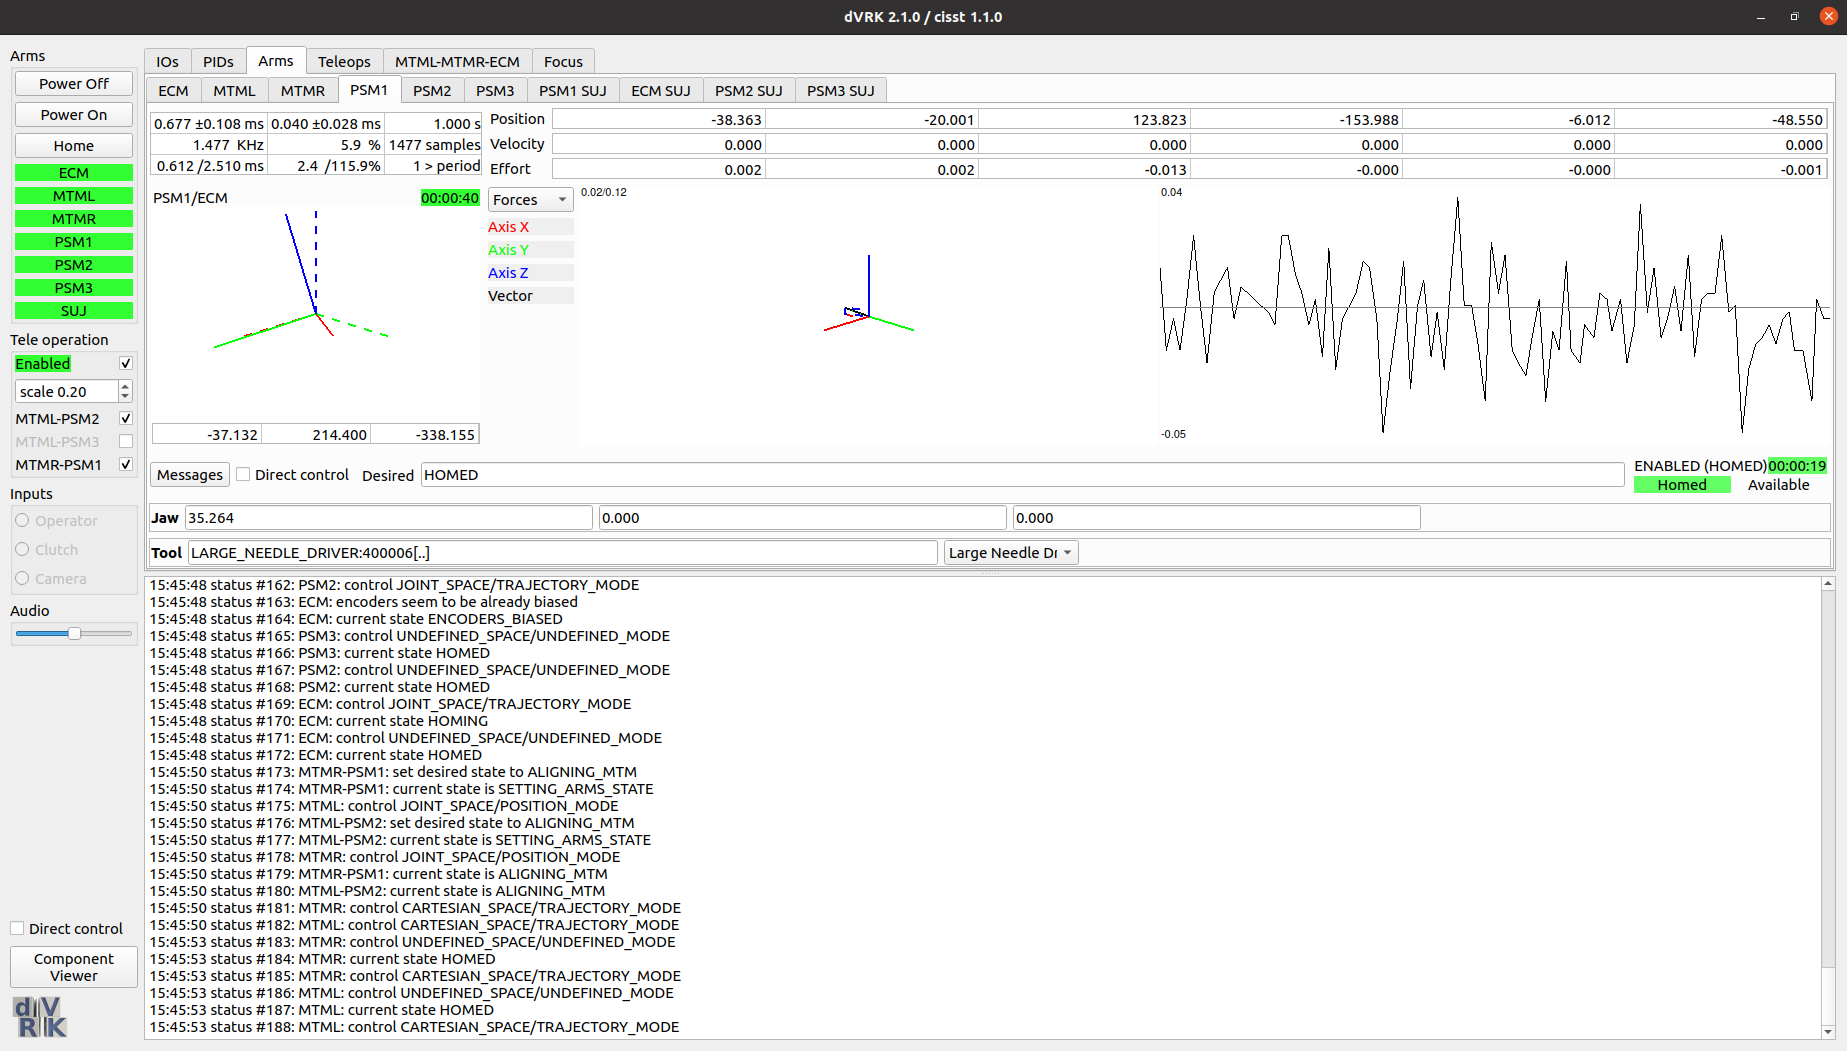
\includegraphics[width=0.95\linewidth]{figures/console_example.png}
    \caption{expected GUI}
    \label{fig:gui_console}
\end{figure}

Click \texttt{power on} and then click \texttt{home}. If all the blocks turn out to be green, then you are good to move forward.

\subsection{ROS 2}

For dVRK in ROS 2, most of the procedures are identical to the procedures for ROS 1. The major differences are:

\begin{itemize}
    \item different dVRK configuration folders as shown in section 3.1.1
    \item different commands for running the ROS consoles and no \texttt{roscore}
\end{itemize}

For ROS 2, please run the following commands when you are in the dVRK configuration folder:

\begin{minted}{bash}
$ ros2 run dvrk_robot dvrk_console_json -j console-[code name].json -p [timestep]
\end{minted}

The expected GUI is the same as the one shown in \autoref{fig:gui_console}.

\section{HRSV Activation}

If you are using DeckLink Duo frame grabber, then please check the instruction in \url{https://github.com/jhu-dvrk/dvrk-ros/blob/devel/dvrk_robot/video.md}. This method is using \texttt{gscam} and \texttt{gstreamer} to obtain the image and publish to ROS image topics.

If you are using SDI-to-USB3 frame grabber, you can also use ROS \texttt{cv\_camera} package to obtain the images and publish to ROS image topics. You may find the ROS launch file following the baseline instruction at WPI local enviroment. Alternatively, you can create your own launch file referring to the launch file shown in \autoref{fig:ros_cvcamera}:

\begin{figure}[H]
    \centering
    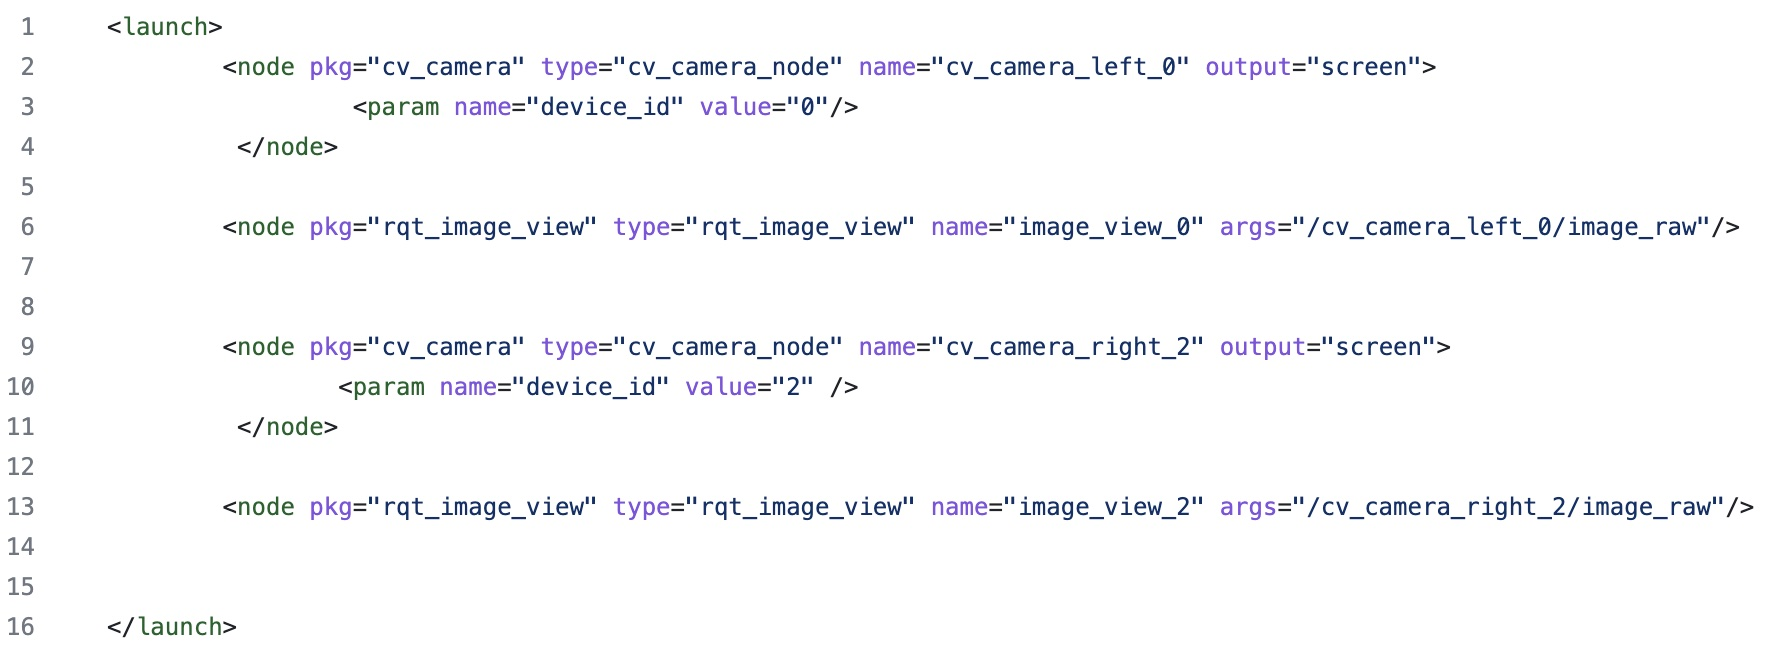
\includegraphics[width=0.95\linewidth]{figures/roslaunch_cvcamera.jpg}
    \caption{ROS launch file example}
    \label{fig:ros_cvcamera}
\end{figure}

As shown in line 3 and 10, the left camera is \texttt{\slash dev\slash video0} and the right camera is \texttt{\slash dev\slash video2}. Nevertheless, we have not forced a udev rule to identify the USB cables for cameras at WPI. Therefore, if you reconnect the USB cables, you may have a chance to reverse the video ID. To confirm the camera IDs are correct, you may need to run the ROS launch firstly and push the \texttt{bar code} button on the camera control unit of the left camera. If the shown camera left figure turns to be a barcode, then you are good to go. Otherwise, you can switch the codes at line 3 and 10.

Eventually, make sure that you drag the image consoles to the HRSV extended monitors.

\chapter{dVRK Baseline at WPI}
\label{ch: baseline}

\section{Hardware Check}

Please follow the instruction in \autoref{ch: hardware}. Check all the hardware are connected properly and powered on.

Release the ESTOP before running the full system of dVRK.

In addition, you may need to check the camera ID if you are worried whether your flipped the camera. Generally, the left camera is \texttt{\slash dev\slash video0} and the right camera is \texttt{\slash dev\slash video2}. Nevertheless, we have not forced a udev rule to identify the USB cables for cameras at WPI. Therefore, if you reconnect the USB cables, you may have a chance to reverse the video ID. To confirm the camera IDs are correct, you can visualize the images via VLC using \texttt{capturing device} firstly and push the bar code button on the camera control unit of the left camera. If the shown camera left figure turns to be a barcode, then you are good to go. Otherwise, you can switch the codes at line
3 and 10.

\section{Software Run}

\subsection{Connection Check}

Firstly, make sure all control boxes are connected to the computer. You may run following command in a terminal to check:

\begin{minted}{bash}
$ qladisp
\end{minted}

If you can see 13 boards are connected as shown in \autoref{fig:qladisp}, then it means that all connections work fine. 

Then, you can run following command in the terminal:

\begin{minted}{bash}
$ qlacommand -c close-relays
\end{minted}

This command is to enable the power of the control boxes. At the same time, you should hear the sound of activated fans. If not, please go back to check the cable connections, power and E-stop. This manual activation of power helps if the SUJ does not power on properly sometimes.

\subsection{ROS 1}

Firstly, you need to activate ROS master via running following command in the terminal:

\begin{minted}{bash}
$ roscore
\end{minted}

Then, you need to enable the endoscope image system with ROS 1. At the local environment, please run following command in a new terminal:

\begin{minted}{bash}
$ cd ~/cristina_ws/src/irb/launch
$ roslaunch camera.launch
\end{minted}

Alternatively, if the camera launch file cannot be found or you would like to make a customized camera launch file. Then, please go ahead to take \autoref{fig:ros_cvcamera} as a reference or template.

Eventually, you can head to the dVRK configuration folder as shown in \autoref{ch: Software} section 3.1.1, then you can run the following command in the terminal to enable the full system teleoperation with 1000Hz refreshing rate:

\begin{minted}{bash}
$ rosrun dvrk_robot dvrk_console_json -j console-SUJ-ECM-MTMR-PSM1-MTML-PSM2-PSM3-Teleop.json
-p 0.001
\end{minted}

For suturing user study, please go with following command (also 1000Hz):

\begin{minted}{bash}
$ rosrun dvrk_robot dvrk_console_json -j console-SUJ-ECM-MTMR-PSM1-MTML-PSM3-Teleop.json
-p 0.001
\end{minted}

If you only run with AMBF simulation, please go with following command:

\begin{minted}{bash}
$ rosrun dvrk_robot dvrk_console_json -j console-MTML-MTMR.json -p 0.001
\end{minted}

\subsection{ROS 2}

The endoscope image system with ROS 2 is currently not available yet. Therefore, you can only go with VLC to visualize the endoscope images.

Then, you can go to the dVRK configuration folder for ROS 2 as shown in \autoref{ch: Software} section 3.1.2 and run following command in the terminal to enable the full system teleoperation with 1000 Hz refreshing rate:

\begin{minted}{bash}
$ ros2 run dvrk_robot dvrk_console_json -j console-SUJ-ECM-MTMR-PSM1-MTML-PSM2-PSM3-Teleop.json
-p 0.001
\end{minted}

For two arm teleoperation for suturing, please go with following command:

\begin{minted}{bash}
$ ros2 run dvrk_robot dvrk_console_json -j console-SUJ-ECM-MTMR-PSM1-MTML-PSM3-Teleop.json
-p 0.001
\end{minted}

\chapter{How to Run Teleoperation}
\label{ch: Teleop}

\section{Move SUJ Manually}

There are four arms attached to the SUJ: ECM, PSM1, PSM2 and PSM3. Except for PSM3, all the other arms shared the same moving technique.

\subsection{PSM1 and PSM2}

As long as you have activated the SUJ, you can move the base of PSM 1 and 2 freely automatically. For example, if you are under dVRK configuration folder and run following commands: 

\begin{minted}{bash}
$ rosrun dvrk_robot dvrk_console_json -j console-SUJ-***.json
\end{minted}

Then push the button located at the SUJ PSM handle shown in \autoref{fig:psm_handle}, you are free to move the PSM 1 and 2 around.

\begin{figure}[H]
    \centering
    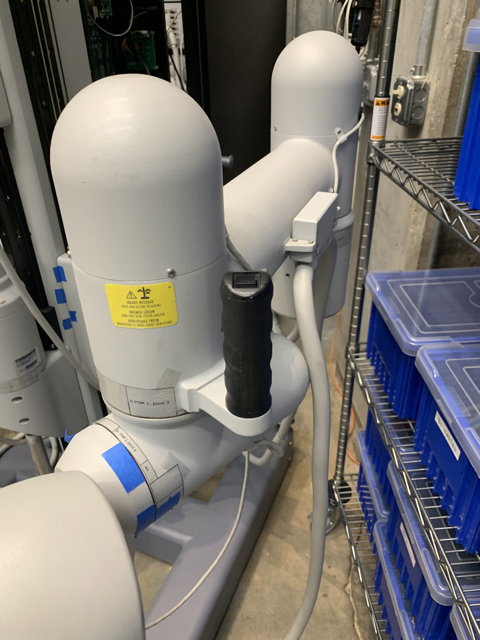
\includegraphics[width=0.4\linewidth]{figures/PSM_handle.png}
    \caption{SUJ PSM handle}
    \label{fig:psm_handle}
\end{figure}

\subsection{ECM}

For moving the base of ECM, you have to enable the power of ECM firstly. For example, if you are under dVRK configuration folder and run following commands: 

\begin{minted}{bash}
$ rosrun dvrk_robot dvrk_console_json -j console-SUJ-ECM-***.json
\end{minted}

Then push the button located at the SUJ ECM handle shown in \autoref{fig:ecm_handle}, you are free to move the base of ECM around.

\begin{figure}[H]
    \centering
    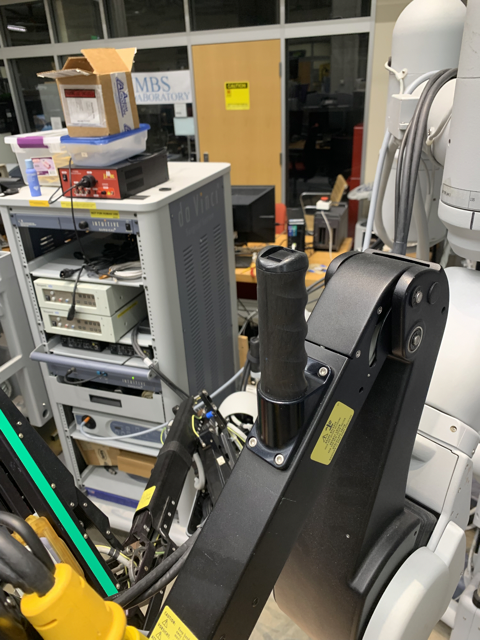
\includegraphics[width=0.6\linewidth]{figures/ECM_handle.png}
    \caption{SUJ ECM handle}
    \label{fig:ecm_handle}
\end{figure}


\subsection{PSM3}

For moving the base of PSM3, you have to enable the power of PSM 3 firstly. For example, if you are under dVRK configuration folder and run following commands: 

\begin{minted}{bash}
$ rosrun dvrk_robot dvrk_console_json -j console-SUJ-***-PSM3-***.json
\end{minted}

Then push the button located at the SUJ PSM3 handle shown in \autoref{fig:psm3_handle}, you are free to move the base of PSM3 around.

\begin{figure}[H]
\centering
\subfloat[Horizontal movement handle]{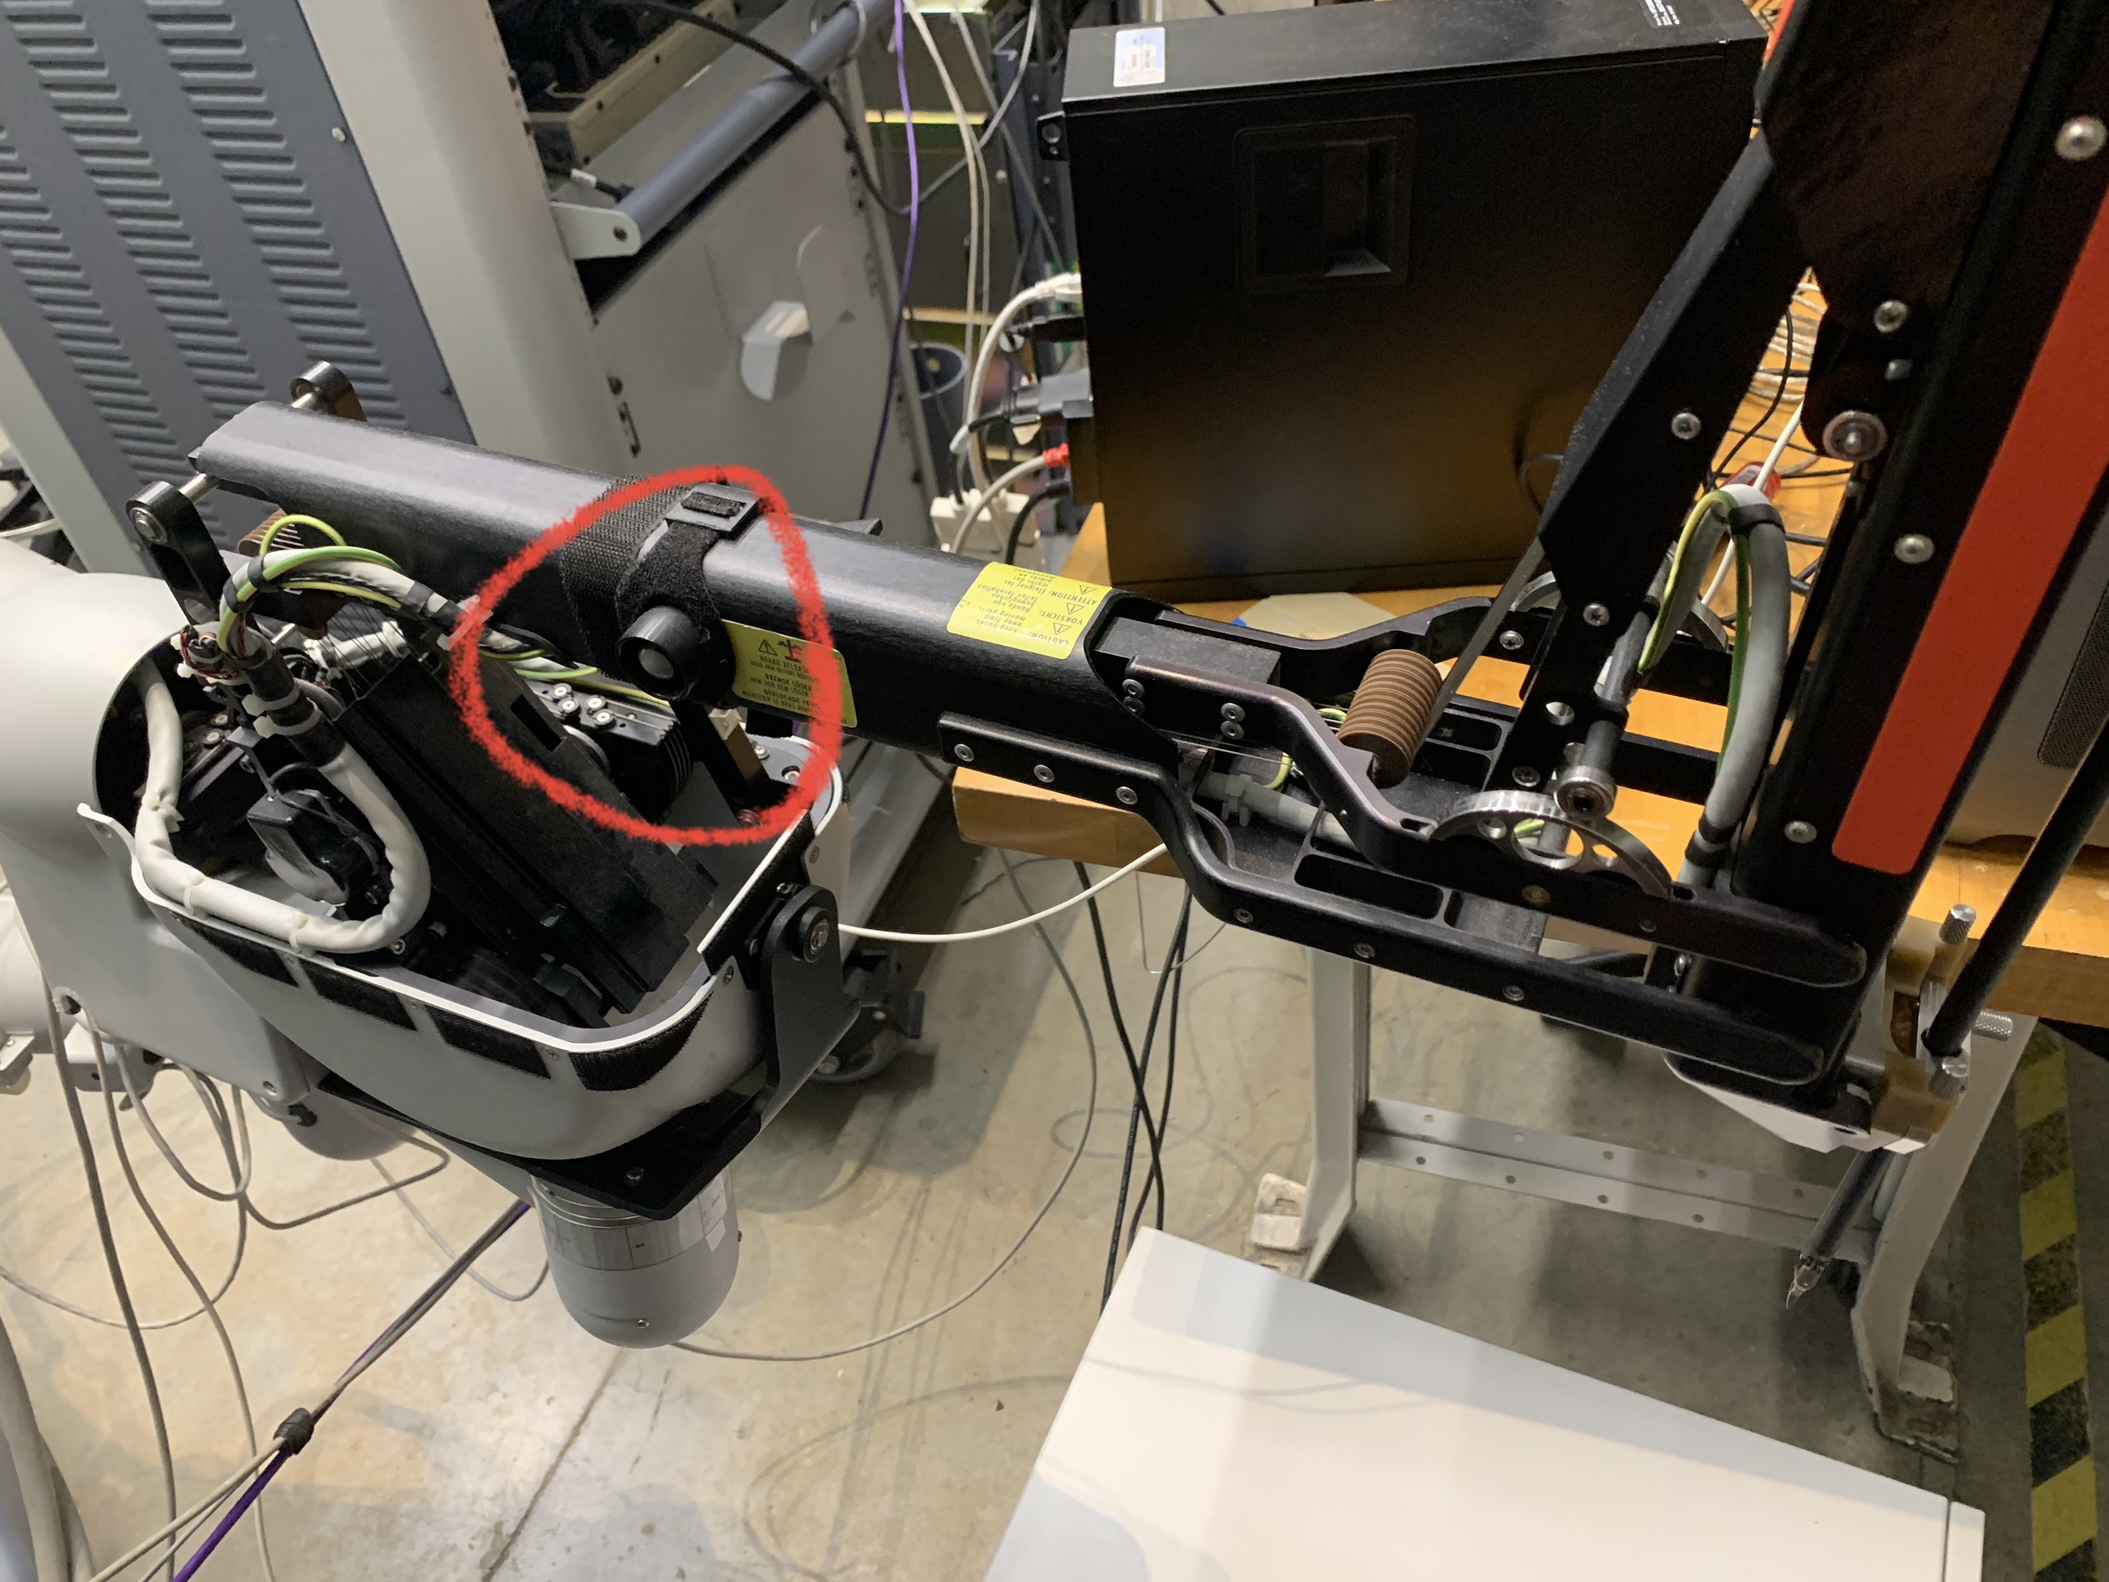
\includegraphics[width=0.45\linewidth, height=5.5cm]{figures/PSM3_handle1.jpg}}
\hfil
\subfloat[Vertical movement handle]{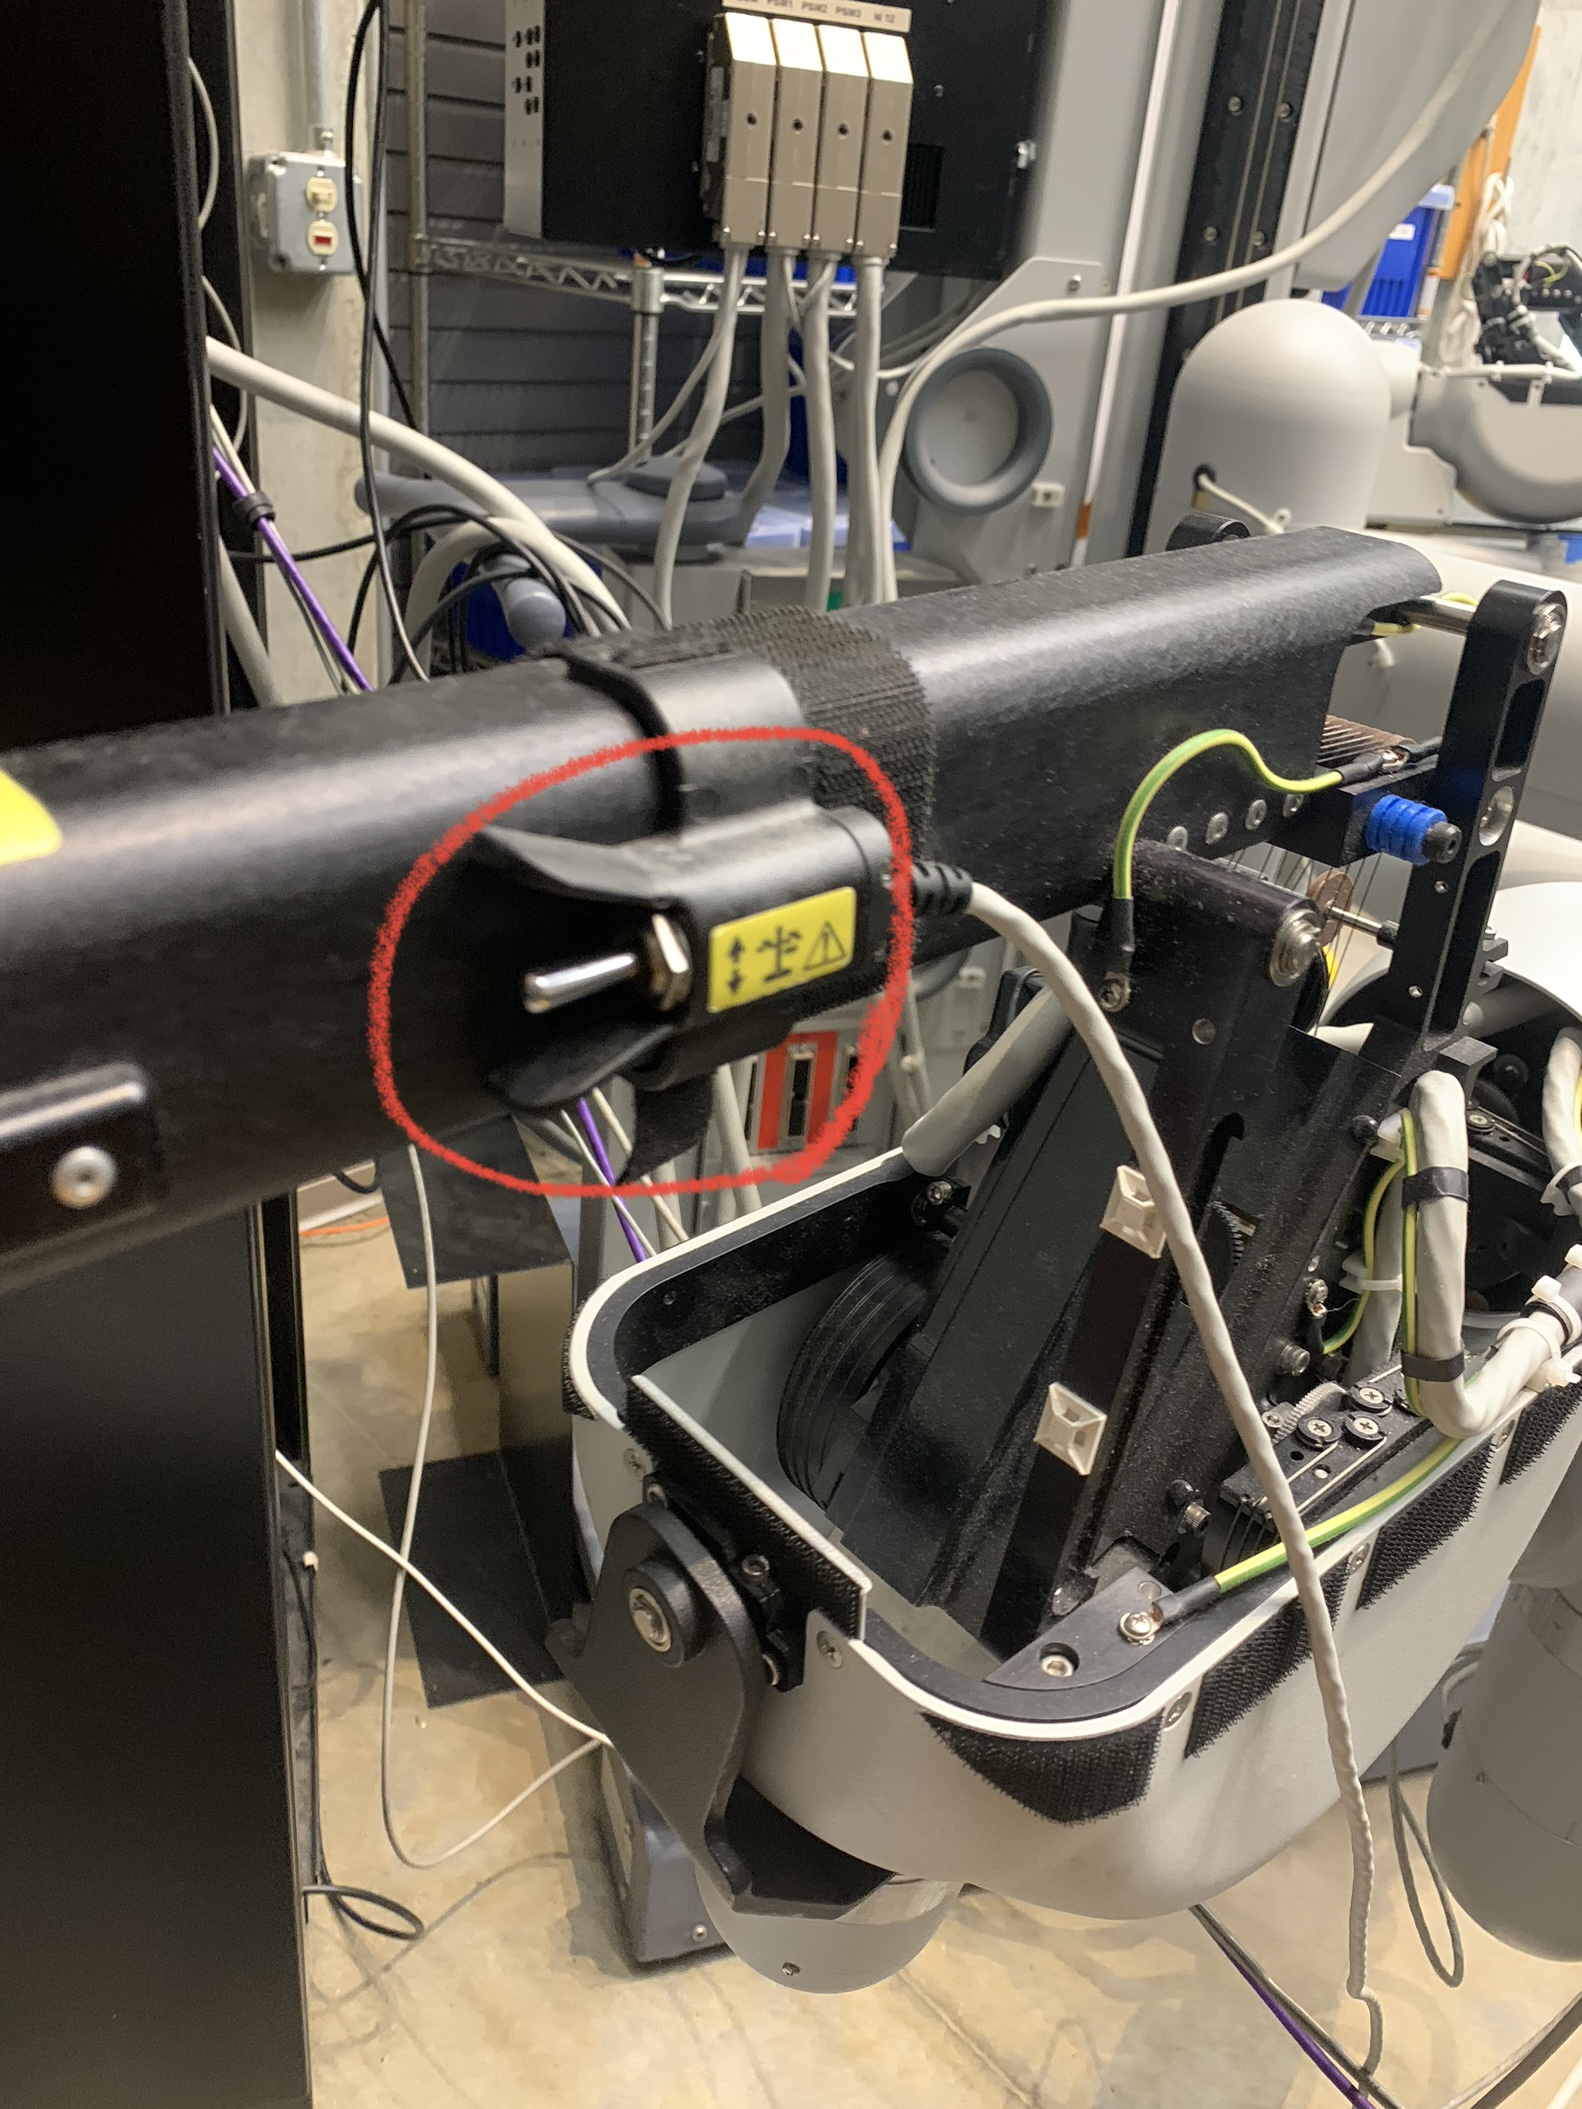
\includegraphics[width=0.45\linewidth, height=5.5cm]{figures/PSM3_handle2.jpg}}
\caption{SUJ PSM3 handle}
\label{fig:psm3_handle}
\end{figure}

\section{Move Robot Arms Manually}

In section 5.1, we introduce how to move the base of robot arms via SUJ. In this section, we would like to introduce how to move the robot arms themselves. The pre-requirement of moving the arms is to enable the power of corresponding arm. Then, you can find a white button at the top of the arms as shown in \autoref{fig:arm_button}. When you press this button, you can move the arms freely.

\begin{figure}[H]
\centering
\subfloat[PSM button]{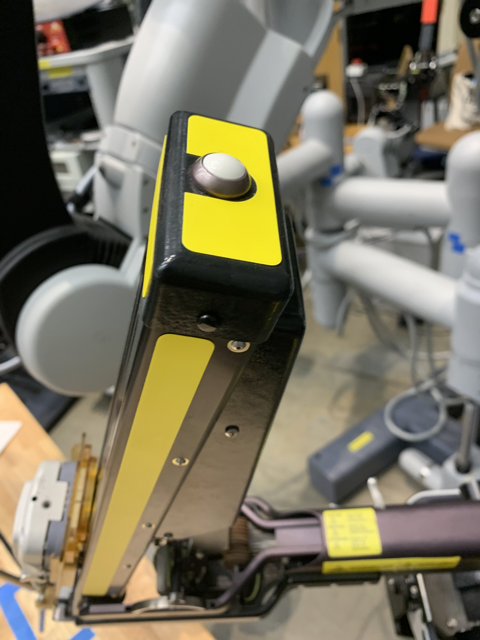
\includegraphics[width=0.45\linewidth]{figures/PSM_button.png}}
\hfil
\subfloat[ECM button]{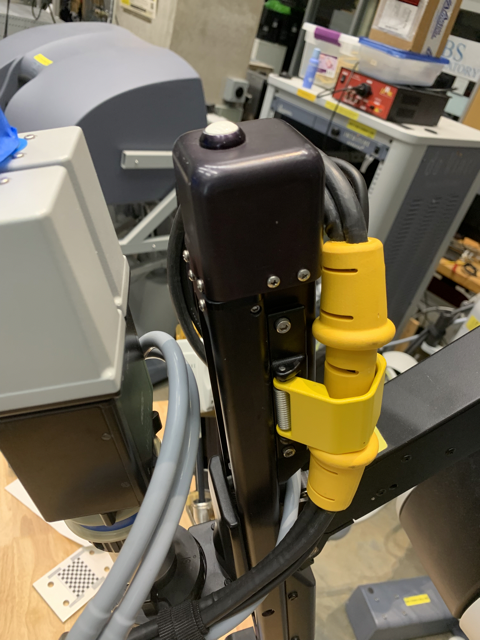
\includegraphics[width=0.45\linewidth]{figures/ECM_button.png}}
\caption{Buttons on different robot arms}
\label{fig:arm_button}
\end{figure}

\section{Foot Pedal}

You may set up your own foot pedal following the instruction in the given link: \url{https://github.com/jhu-dvrk/sawIntuitiveResearchKit/wiki/FootPedals}. Alternatively, you may obtain a foot pedal shown in \autoref{fig:origin_footpedal} with the hardware of dVRK.

\begin{figure}[H]
\centering
\subfloat[WPI foot pedal]{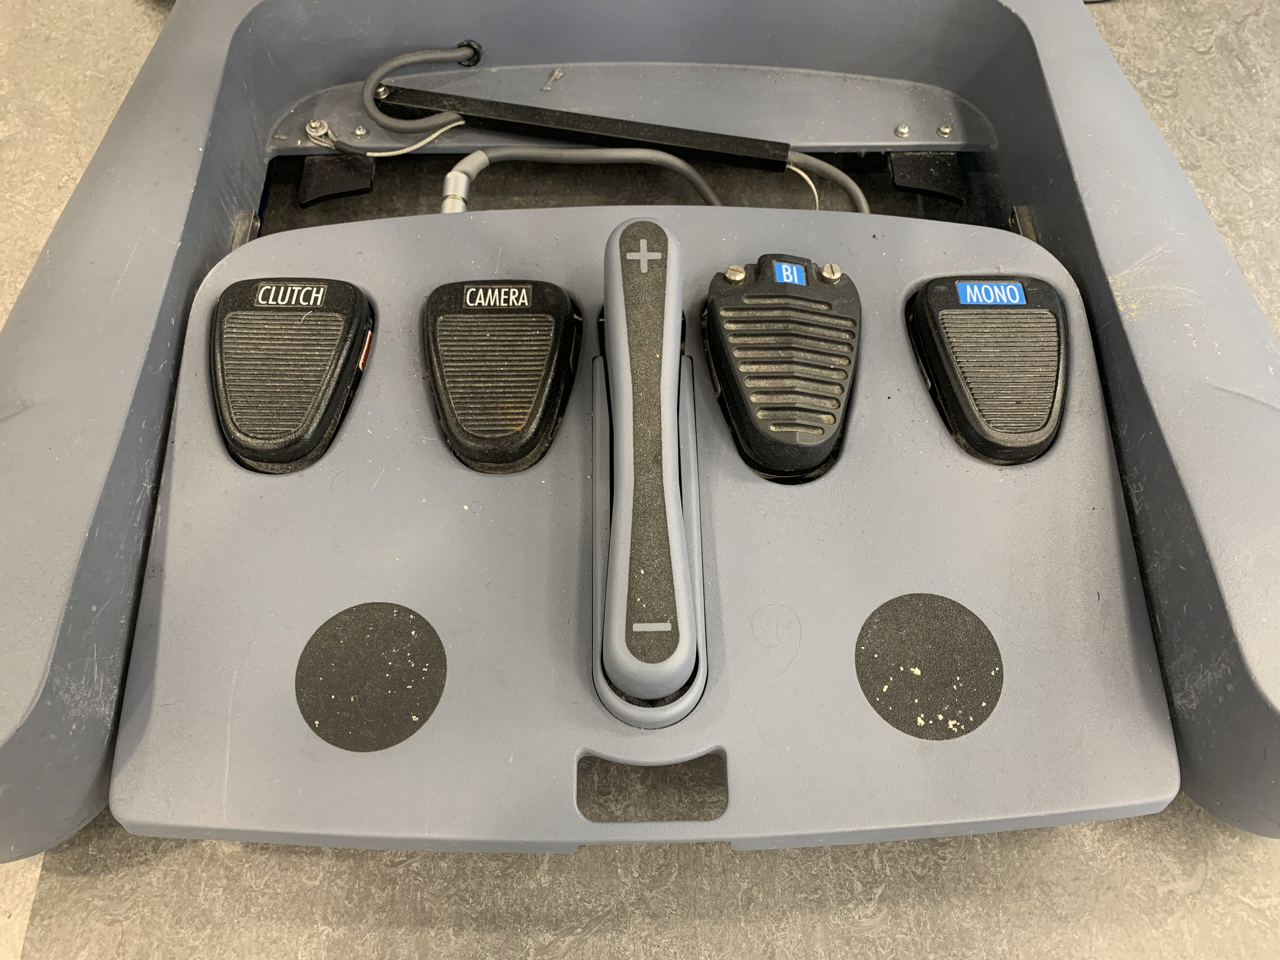
\includegraphics[width=0.45\linewidth]{figures/footpedal_wpi.png}}
\hfil
\subfloat[JHU foot pedal]{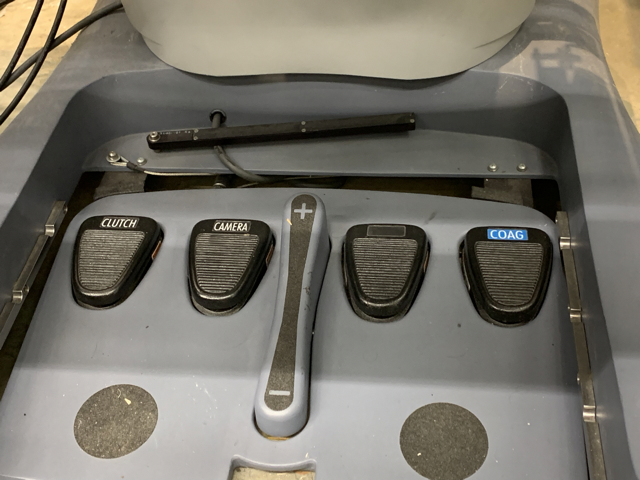
\includegraphics[width=0.45\linewidth]{figures/footpedal_jhu.png}}
\caption{Foot pedal come with dVRK}
\label{fig:origin_footpedal}
\end{figure}

Assume that you have ran the full system of dVRK with teleoperation enabled.

\subsection{Endoscope Focus Modification}

If you would like to modify the focus of the endoscope, you can use the button in the middle of the foot pedal. It is a straightforward mapping from focus control box to the foot pedal button. The pre-requirement for this operation is the cable connection discussed in section 2.1.4 in \autoref{ch: hardware}.

\subsection{Teleoperate PSM}

Each MTM is corresponded to one PSM. The match between MTMs and PSMs is shown as following:

\begin{itemize}
    \item MTMR - PSM1
    \item MTML - PSM2 or PSM3
\end{itemize}

The teleoperation is an one-to-one mapping. It maps your movements at MTM to PSM tool tip with a given scale (default to be 0.2).

The operation of the foot pedal for PSM teleoperation is shown as following:

\begin{itemize}
    \item hold MONO/COAG pedal: enable the teleoperation
    \item hold MONO/COAG pedal and CLUTCH pedal: Move the MTM freely without moving PSM, leverage to extend your work space.
    \item press CLUTCH pedal without holding MONO/COAG pedal: switch the control pairs for PSM2 and PSM3 if enabling all three PSMs.
\end{itemize}

It may take some time to find the inverse kinematic of MTM if you move too fast or move around a singularity. At those times, the teleoperation is disabled for a while. If this happens, please hold MONO/COAG pedal and wait for MTM to self-adjust to the desired pose. If waiting doesn't fix the problem, you can also restart the console to fix it.

\subsection{Teleoperate ECM}

Two MTMs are corresponded to one ECM. Imagine you are operating a wheel with two hands, the teleoperation follows this manner.

The operation of the foot pedal for ECM teleoperation is shown as following:

\begin{itemize}
    \item hold MONO/COAG pedal and CAMERA pedal: enable the teleoperation
    \item hold MONO/COAG pedal and CLUTCH pedal: Move the MTM freely without moving ECM, leverage to extend your work space or reset MTM poses.
\end{itemize}

Please avoid any sudden movements. If your movements are too swift, the ECM would be hard to follow and trigger a shutdown because of the inconsistency between the encoder and the potentionmeter.



% \chapter{Other Nonfunctional Requirements}
% \label{Other Nonfunctional Requirements}

% \section{Performance Requirements}
% \section{Safety Requirements}
% \section{Security Requirements}
% \section{Software Quality Attributes}
% \section{Business Rules}

\chapter{Common Q \& A}
\label{ch: Q&A}

\section{Cannot Detect the Board}

\subsection{All Boards not Detected}

Firstly, please ensure that all control boxes connection and hardware setup are valid following the instruction in \autoref{ch: hardware}. 

Then, unplug the firewire from the desktop. Wait for 5 seconds. Replug the firewire back to the desktop. Wait for 5 seconds. Then check the board detection with running following command is a new terminal:

\begin{minted}{bash}
    qladisp
\end{minted}

If this operation cannot solve the problem, please check the discussion in \url{https://github.com/jhu-dvrk/sawIntuitiveResearchKit/discussions} or create a new issue in this discussion board.

\subsection{Some Boards not Detected}

If you can detect some of the boards, please firstly check the board ID and refer to \autoref{tab:arm_config} to find out the first control box which is not detected. Then, unplug the firewire from the control box. Wait for 5 seconds. Replug the firewire back to the control box. Wait for 5 seconds. Then check the board detection with running following command is a new terminal:

\begin{minted}{bash}
    qladisp
\end{minted}

If this operation cannot solve your issue, you may open the control box to check whether the internal cables and FPGA/QLA board work or not. If one of them is broken, you may replace it if you have some spare components. 

If all described operations still cannot solve your problem, please check the discussion in \url{https://github.com/jhu-dvrk/sawIntuitiveResearchKit/discussions} or create a new issue in this discussion board.

\section{Teleoperation Stuck}

Teleoperation stuck means that you can still move MTMs but the PSMs are not following under teleoperation mode.

Firstly, you can check the GUI console to ensure everything is still working. If not, simply click \texttt{power on}, then click \texttt{home} and check \texttt{Enabled} under \texttt{Tele operation} box can save the problem. Alternatively, you can also close the dVRK robot console and restart in the terminal. I will list some tricks for recovering from the stuck status.

\subsection{Trick 1}

Hold MONO/COAG pedal and wait for MTM to stabilize. Then you can attempt to recover the teleoperation for PSMs.

\subsection{Trick 2}

Release all pedals and buttons on the foot pedal. Wait for 5 seconds. Then, hold MONO/COAG button and attempt to open and close the MTM grippers. It may allow you recover your teleoperation.

\subsection{Trick 3}

If you can visually check that the PSM is in a singularity of in a strange pose. You can manually move your PSM back to a regualr pose via the instruction in section 5.2 in \autoref{ch: Teleop}. This may help you recover your teleoperation.

\subsection{Trick 4}

Close and restart the dVRK robot GUI console. Reboot should always be helpful.

\section{MTM Misalignment}

Sometimes, the MTM grippers can be misaligned when you home the MTMs as shown in \autoref{fig:mtm_misalgin}.

\begin{figure}[H]
\centering
\subfloat[Misaligned grippers]{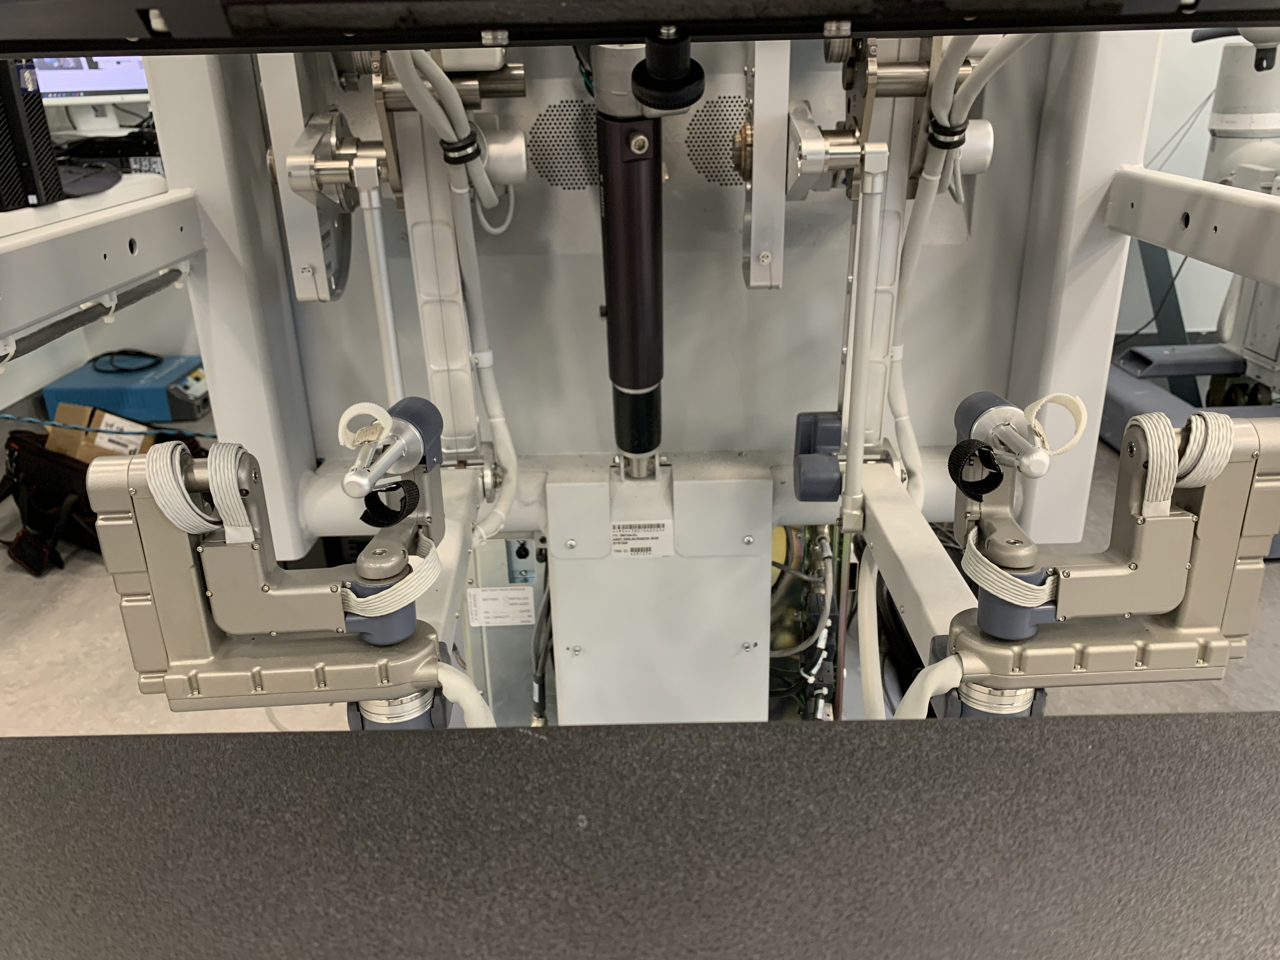
\includegraphics[width=0.45\linewidth]{figures/mtm_misalign.png}}
\hfil
\subfloat[Aligned grippers]{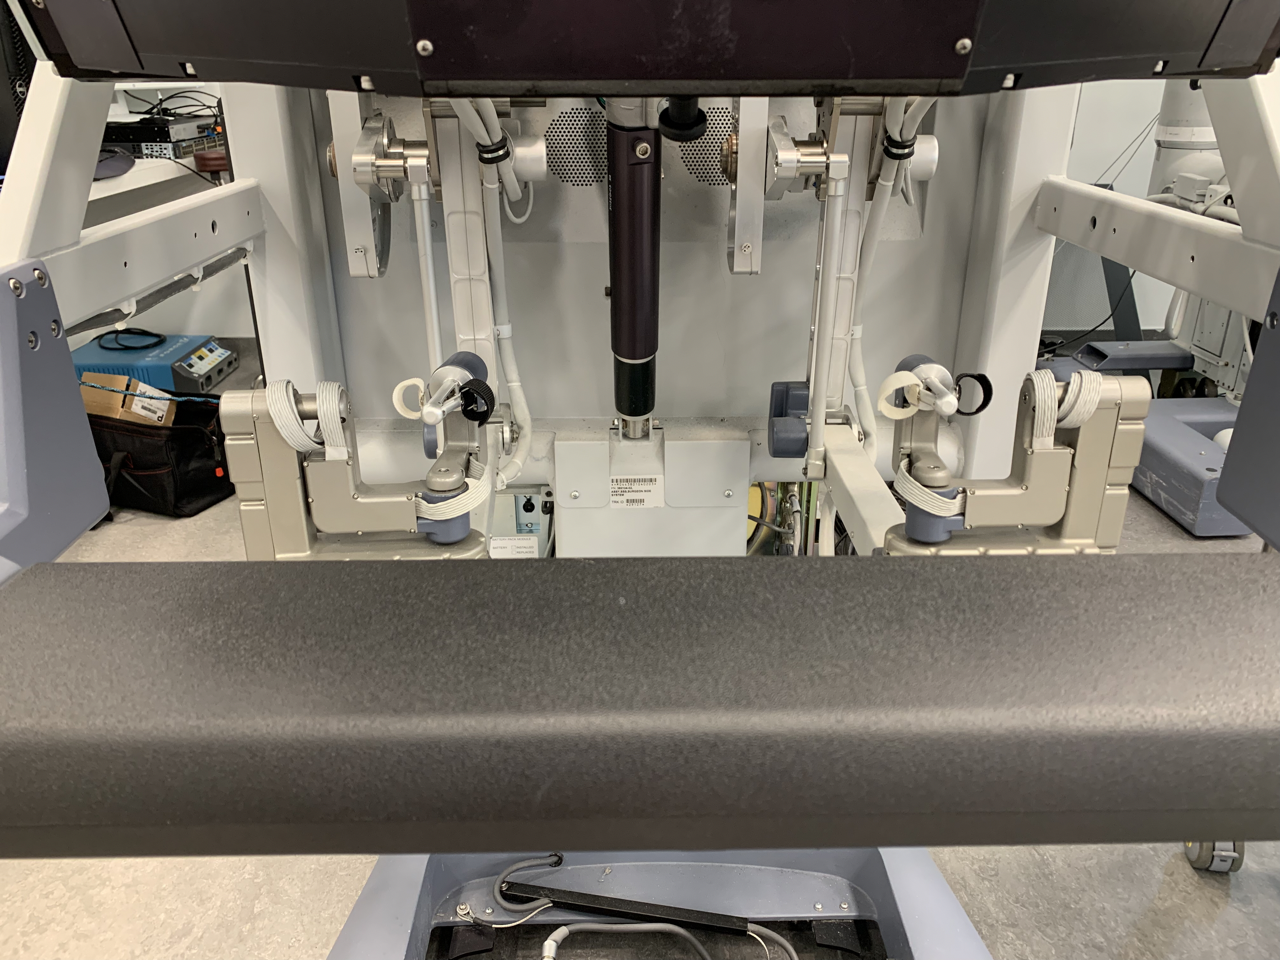
\includegraphics[width=0.45\linewidth]{figures/mtm_fixed.png}}
\caption{MTM Misalignment}
\label{fig:mtm_misalgin}
\end{figure}

Sometimes, a current calibration as instructed in section 2.3.4 in \autoref{ch: hardware} can solve the problem. 

Nevertheless, if a simple current calibration cannot solve the problem. We can use some advance techniques to solve this issue as shown in \url{https://github.com/jhu-dvrk/sawIntuitiveResearchKit/wiki/Calibration#calibrating-scales}. 

Taking MTML as an example, run following command in a new terminal under the path of dVRK configuration folder:

\begin{minted}{bash}
    rosrun dvrk_robot dvrk_console_json -j console-MTML.json -i ../ros-io-MTML.json -C
\end{minted}

It will enable a dVRK GUI console and click \texttt{home} button.

Then, open a new terminal under the same folder path and run:

\begin{minted}{bash}
    rosrun dvrk_robot dvrk_calibrate_potentiometers.py -t scale -a MTML -c sawRobotIO1394-MTML-33100.xml
\end{minted}

Make sure you have enough free space for MTM to run this code. Then, just follow the instructions in the terminal.

After the scale calibration, your problem supposes to be solved.


\clearpage

\printbibliography

% \begin{appendices}
% % \chapter{Glossary}
% % \chapter{Analysis Models}
% \chapter{To Be Determined List}


% \end{appendices}


